\documentclass[usenatbib]{mn2e}
\usepackage{amsmath} 
\usepackage{amssymb} 
\usepackage{graphics}
\usepackage{graphicx}
\usepackage{epsfig}  
\def\be{\begin{equation}}
\def\ee{\end{equation}}
\def\ba{\begin{eqnarray}}
\def\ea{\end{eqnarray}}

\newcommand{\documentname}{paper~}
\newcommand{\match}{{\tt match}~}
\newcommand{\apj}{ApJ}  
\newcommand{\apjs}{ApJS}  
\newcommand{\apjl}{ApJL}  
\newcommand{\aj}{AJ}  
\newcommand{\mnras}{MNRAS}  
\newcommand{\mnrassub}{MNRAS accepted}  
\newcommand{\aap}{A\&A}  
\newcommand{\aaps}{A\&AS}  
\newcommand{\araa}{ARA\&A}  
\newcommand{\nat}{Nature}  
\newcommand{\physrep}{PhR}
\newcommand{\pasp}{PASP}    
\newcommand{\pasj}{PASJ}    

\newcommand{\kms}{\,km~s$^{-1}$}
\def\squig{\sim\!\!}
\newcommand{\LCDM}{$\Lambda$CDM~}
\newcommand{\beq}{\begin{eqnarray}}  
\newcommand{\eeq}{\end{eqnarray}}   
\newcommand{\zz}{$z\sim 3$} 
\newcommand{\avg}[1]{\langle{#1}\rangle}  
\newcommand{\ly}{{\ifmmode{{\rm Ly}\alpha}\else{Ly$\alpha$~}\fi}}
\newcommand{\hMpc}{{\ifmmode{h^{-1}{\rm Mpc}}\else{$h^{-1}$Mpc }\fi}}  
\newcommand{\hGpc}{{\ifmmode{h^{-1}{\rm Gpc}}\else{$h^{-1}$Gpc }\fi}}  
\newcommand{\hmpc}{{\ifmmode{h^{-1}{\rm Mpc}}\else{$h^{-1}$Mpc }\fi}}  
\newcommand{\hkpc}{{\ifmmode{h^{-1}{\rm kpc}}\else{$h^{-1}$kpc }\fi}}  
\newcommand{\hMsun}{{\ifmmode{h^{-1}{\rm
        {M_{\odot}}}}\else{$h^{-1}{\rm{M_{\odot}}}$}\fi}}   
\newcommand{\hmsun}{{\ifmmode{h^{-1}{\rm
        {M_{\odot}}}}\else{$h^{-1}{\rm{M_{\odot}}}$}\fi}}   
\newcommand{\Msun}{{\ifmmode{{\rm {M_{\odot}}}}\else{${\rm{M_{\odot}}}$}\fi}}  
\newcommand{\msun}{{\ifmmode{{\rm {M_{\odot}}}}\else{${\rm{M_{\odot}}}$}\fi}}  
\newcommand{\lya}{{Lyman$\alpha$~}}
\newcommand{\clara}{{\texttt{CLARA}}~}
\newcommand{\rand}{{\ifmmode{{\mathcal{R}}}\else{${\mathcal{R}}$ }\fi}}  
\newcommand{\Lsun}{\mbox{\,$L_{\odot}$}}
\newcommand{\like}{\mathscr{L}}
\newcommand{\bftheta}{\mathbf{\Theta}}
\newcommand{\degree}{\ensuremath{^\circ}}
\def\spose#1{\hbox to 0pt{#1\hss}}
\def\simlt{\mathrel{\spose{\lower 3pt\hbox{$\mathchar"218$}}
     \raise 2.0pt\hbox{$\mathchar"13C$}}}
\def\simgt{\mathrel{\spose{\lower 3pt\hbox{$\mathchar"218$}}
     \raise 2.0pt\hbox{$\mathchar"13E$}}}
\font\smcap=cmcsc10

\begin{document}

\title[Halo mass and occupation fraction for LAEs at
  $z=3.1$]{Constraints on the mass and occupation
  fraction of dark matter halos hosting Lyman-alpha emitters
  at $z\sim 3$}    
\author[~J.~E. Forero-Romero and J. Mejia]{
\parbox[t]{\textwidth}{\raggedright 
Jaime E. Forero-Romero$^{1}$ and
Julian Mej\'ia-Restrepo$^{2}$ 
}
\vspace*{6pt}\\
$^{1}$ Departamento de F\'{i}sica, Universidad de los Andes, Cra. 1
No. 18A-10, Edificio Ip, Bogot\'a, Colombia \\
$^{2}$ Departamento de Astronom\'{i}a, Universidad de Chile, Camino el
Observatorio 1515, Santiago, Chile} 

\maketitle

\begin{abstract}
%
We derive constraints on the mass and occupation fraction of dark
matter halos hosting \ly Emitting galaxies (LAEs) at a redshift of
$z=3.1$, by comparing the number density and the angular
correlation function between mock and observed fields. The mock fields
are constructed in a large cosmological N-body simulation using a
model where a dark matter halo can only host one LAE with a
probability $f_{\rm occ}$ if its mass is within the mass range
delimited by two threshold values  $M_{\rm min}$ and $M_{\rm max}$. We
conclude that the number density and spatial clustering information
available from observations is not sufficient to derive a unique and narrow set of
values for the parameters in the model. We find three different
families of models based on their mass range $\Delta M \equiv
\log_{10}M_{\rm max} - \log_{10} M_{\rm min}$ dex and occupation
fraction $f_{\rm occ}$.  However, there is a dominant familiy composed
by models with a narrow mass range $\Delta M<1.0$ dex, a low
occupation fraction $f_{\rm occ}\leq 0.3$ and a maximum mass $M_{\rm
  max}< 10^{12}$\hMsun.  This finding suggests that the most massive
dark matter halos at that epoch do not host the brightest LAEs. This
also gives support to observational evidence concluding that only a
small fraction of star forming galaxies can be actually detected as
LAEs. We provide tables and mock catalogs for the successful models. 
\end{abstract}

\begin{keywords}
{cosmology: theory – cosmology: large-scale structure of universe –
  galaxies: formation – galaxies: high-redshift – galaxies: statistics
  – galaxy: haloes} 
\end{keywords}


\section{Introduction}

Lyman-$\alpha$ emitting galaxies (LAEs) have become in the last decade a 
central topic in studies of structure formation in the Universe. They 
are helpful in a diverse range of fields. LAEs can
be used as probes of reionization \citep{Dijkstra11}, tracers of
large scale structure \citep{Koehler2007}, 
signposts for low metallicity stellar populations and markers of the
the galaxy formation process through cosmic history \citep{ForeroRomero2012}.  


At the same time, theoretical and observational developments have
contributed to the emergence of a paradigm to describe structure
formation in a cosmological context. In this context it is considered
that dominant matter content of the Universe is to be found in dark
matter, whereby each galaxy is hosted by larger dark matter structure
known as a halo. 

Most models of galaxy formation find that the mass of the halo can be
used to predict properties of the galaxy such as its stellar mass and
star formation rate \citep{Behroozi2012}. Processes that regulate the
star formation cycle are also though to be strongly dependent on its
mass. Furthermore, the spatial clustering of galaxies on large scales
is entirely dictated by the halo distribution.  For the reasons
mentioned above, finding the typical dark matter halo mass hosting
LAEs represents a significant step forward to understand the nature of
this population in the context of Lambda Cold Dark Matter
($\Lambda$CDM) paradigm.  

Some theoretical approaches to this problem have been based on
ab-initio approach modeling. Starting from the DM halo population, the
corresponding intrinsic star formation properties are inferred
together with other statistics such as the luminosity function, the
correlation function and the equivalent width distributions. Such
modelling has been implemented from analytic considerations,
semi-analytic models  and  full N-body hidrodynamical simulations
\citep{Laursen2007, Dayal2009, ForeroRomero2011, Yajima2012, Orsi2012, Soler2012}. 

Added to the uncertainties in the astrophysical processes describing
star formation in galactic populations, a highly debated step in this
approach is the calculation of the fraction of \ly photons
that escape the galaxy to the observer. Given the resonant nature of
the \lya line, the radiative transfer of \ly is sensitive to the
density, temperature, topology and kinematics of the neutral Hydrogen
in the interstellar medium (ISM) \citep{Neufeld1991, ForeroRomero2011, Dijkstra2012,
Laursen2013,Orsi2012}.  

This complexity makes the use of monte-carlo simulations for the
radiative transfer a required tool to obtain physically sound results,
although the degeneracy in the physical parameters involved in the
problem makes it difficult to achieve a robust consensus on what is
the theoretical expected value for the \ly escape fraction
at high redshift. 

Our objective in the present \documentname is to use a method to
bypass all the complexity involved in the estimation of the \ly escape
fraction to infer information relevant to the understanding of LAEs in
a cosmological context. The analysis we present is thus based on one
of the most robust prediction of $\Lambda$CDM, namely the clustering
and abudance of dark matter halos. We construct a simple model that
allow us to construct mock catalogs and explore a wide range of
parameters to narrow the mass interval of halos hosting LAEs together
with its occupation fraction. 

Another central point in our study is the explicit inclusion of cosmic
variance effects by using large volume cosmological simulations. This
allows us to go closer to the space of observables and directly
explore the compatibility of a model with observations.

This paper is structured as follows. In the next section we present
the simulation and model used to produce the mock catalogs and the criteria
used to compare them against observations. In \SS \ref{sec:results} we
present the main results in terms of the parameters of our model. We
continue with a discussion of these results under the light of other
observational results for LAEs and abundance matching models for
galaxy formation before presenting our conclusions in \SS
\ref{sec:conclusions}. 

Throughout this \documentname we assume a $\Lambda$CDM cosmology with the
following values for the cosmological parameters, $\Omega_{m}=0.27$,
$\Omega_{\Lambda}=0.73$ and $h=0.70$, corresponding to the matter
density, vacuum density and the Hubble constant in units of 100 km
s$^{-1}$ Mpc$^{-1}$. 

\section{Methodology}

Our method is based on the comparison of observatios and mock
catalogs on the surface number density and the angular correlation
function.  In the next subsections we describe in detail the four key
elements of this workflow. First, we present the observations we take
as a benchmark. Second, the N-body simulation and the halo catalogs we
use. Third, the simplified model that allows us to translated halo
catalogs into mock LAE observations. Fourth, the statistics we use to
compare observational results against our theoretical predictions. 

\subsection{Observational Constraints}

One of the main observational benchmarks we use in this paper is the LAE number
density information at $z=3.1$ obtained by the panoramic narrow-band
survey presented by \cite{Yamada2012} from a survey  conducted with
the Subaru 8.2m telescope and the Subaru Prime Focus Camera, which has
a field of view covering $34\times 27$ arcmin, corresponding to a
comoving scale of $46\times35$ Mpc $h^{-1}$ at $z=3.09$. The narrow
band filter is centered at $4977$ \AA with  $77$\AA width,
corresponding to the redshift range $z=3.062-3.125$ and $41$ Mpc
$h^{-1}$ comoving scale for the detection of the Lyman-$\alpha$ line
centered at $z=3.09$. The authors report a total  $2161$ LAEs with an
observed equivalent width larger than $190$\ over a total survey area
of $2.42$ deg$^{2}$, this corresponds to  average surface number
density of $0.20\pm 0.01$ arcmin$^{-2}$.   

The survey covered four independent fields. The first is the SSA22
field of $1.38$ deg$^2$ with $1394$ detected LAEs, this field has been
known to harbor a region with a large density excess of galaxies. The
second observed region is composed by the fields Subaru/{\it
  XMM-Newton} Deep Survey (SXDS)-North, -Center and -South, with a 
total of $0.58$ deg$^2$ and $386$ LAEs. The third and fourth fields
are the Subaru Deep Field (SDF) with $0.22$ deg$^2$ and $196$ LAEs,
and the field around the Great Observatory Optical Deep Survey North
(GOODS-N) with $0.24$ deg$^2$ and $185$ LAEs. 

There is abundant observational work done on LAEs at redshift $z=3.1$
\citep{Kudritzki2000,Matsuda2005,Gawiser2007,Nilsson2007,Ouchi2008}.
However, we decide to focus on the data from \cite{Yamada2012} because
it has the largest covered area with homogeneous instrumentation
conditions (telescope, narrow band filter), data reduction pipeline
and conditions to construct the LAE catalog. This ensures that the
number density variations among fields are due only to
astrophysical reasons and not different observational conditions or
criteria to construct the catalogs.



\subsection{Simulation and Halo Catalogs}

The Bolshoi simulation \citep{Bolshoi} we use in this paper was
performed in a cubic volume of 250 $h^{-1}$ Mpc on a side. It includes
dark matter distribution is sampled using $2048^{3}$ particles, which
translates into a particle mass of $m_{\rm   p}=1.35\times 10^{8}$
$h^{-1}$ M$_{\odot}$.  The cosmological parameters are consistent with
a WMAP5 and WMAP7 data with a  density $\Omega_{\rm m} = 0.27$,
cosmological  $\Omega_{\Lambda}=0.73$, dimensionless Hubble constant
$h=0.70$, slope of the power spectrum $n=0.95$ and normalization of the
power spectrum$\sigma_{8}=0.82$ \citep{Komatsu2009,Jarosik2011}.  

We use halo catalogs constructed with a Friend-of-Friends (FOF)
algorithm with a linking length of 0.17 times the inter-particle
distance. The minimum halo mass in the models we construct in this \documentname
correspond to groups of $\sim 75$ particles. The catalogs were
obtained from the publicly available Multidark database \footnote{{\tt
    http://www.multidark.org/MultiDark/}} \citep{2011arXiv1109.0003R}.
We focus our work on halos more massive than $1\times 10^{10}$\hMsun
that are resolved with at least $70$ particles.


\subsection{A Model to Populate Halos with LAEs}
\label{subsec:mocks}

In our model a dark matter halo can only host one or zero LAE. 
There are three parameters in the model that decide whether a halo can host a
galaxy or not: the lower and upper bounds for the mass range $M_{\rm min}<
M_{\rm h} < M_{\rm max}$ where LAEs reside and the fraction $f_{\rm
  occ}$ of such halos that effectively host a LAE. We do not assign a
luminosity to each LAE. We are primarily interested in
constraining the halo mass range hosting detectable LAEs under the
conditions defined by \cite{Yamada2012}. In what follows we will describe by
the letter ${\mathcal M}$ a model defined by an specific choice of the
three scalar parameters $M_{\rm min}$, $M_{\rm  max}$ y $f_{\rm occ}$.  


For each model ${\mathcal M}$ we create a set of mock fields from
disjoint volumes in the simulation. Each volume has the same geometry
probed by Suprime-CAM and the narrow band filter, namely rectangular
cuboids of dimensions $46\times 35\times 41$ $h^{-3}$Mpc$^{3}$ where
the last dimension goes in the redshift direction. This corresponds to
a total area of $880$ arcmin$^{2}$ in each mock field. We construct a total
$5\times 7 \times 6=210$ of such volumes from a snapshot in the Bolshoi
simulation. In each mock field a LAE is assigned to the position of a
dark matter halo if the halo mass is in the range allowed by the model
$M_{\rm min}<M_{\rm h}<M_{\rm max}$ and a random variable taken from
an homogeneous distribution $0\leq \xi<1$ is smaller than the occupation
fraction $\xi<f_{\rm occ}$.

Next we construct mock surveys by making groups of $11$ mock fields
out of the $210$ available volumes. In total $15$ mock surveys are
constructed for each model $\mathcal{M}$. The grouping is done in two
different ways. In the first way, called {\texttt match}, we follow
the clustering of the observed fields. From the $11$ mock fields, $7$
are constructed from contiguous fields in the simulation to mimic the
SSA22 region, $3$ are also contiguous between them but not to the first
$7$ fields to mimic the SXDS fields and finally $2$ non-contiguous
fields to imitate the SDF and GOODS-North field. Our main goal with
this selection is to test the impact on the final statistics of having
$7$ clustered fields. The second way to group the mock fields is called {\texttt
  random}, whereby all the $11$ fields are selected in such a way as
to avoid that any two volumes are contiguous.



The second benchmark is the angular correlation function (ACF). The
measurements presented in \citep{Yamada2012} do not report an ACF
measurement. Instead we use the results reported by
\citep{Hayashino2004} on the LAEs observed in the densest field of
SSA22. It is important to keep in mind that there are some differences
between this work and \citep{Yamada2012}. First, the color selection by
\cite{Yamada2012} is less stringent compared to the one by
\cite{Hayashino2004}. Also the EW threshold is different,
\cite{Hayashino2004} uses a cut around $154$\AA \ instead of $190$\AA
\ used by \citep{Yamada2012}


\subsection{Sampling and Selecting Models}

We make a thorough exploration of the parameter space for the models
${\mathcal M}$. $\log_{10} M_{\rm min}$ takes $30$ values from $10.0$ up
to $12.9$ with an even spacing of $0.1$ dex. $\log_{10} M_{\rm max}$
takes values in the same range as $\log_{10}M_{\rm min}$ only with a
displacement of $0.1$ dex in the whole range. The occupation fraction
$f_{\rm occ}$ takes $10$ different values from $0.1$ to $1$ regularly
spaced by $0.1$. In total the number of different models ${\mathcal
  M}$ that are explored is $30 \times 30 \times 10 = 9000$.

For each mock survey generated in a given model ${\mathcal M}$ we
compute the surface density in the $12$ mock fields. We perform a
Kolmogorov-Smirnov (KS) to compare this mock date against the $12$
observational values. From this test we obtain a value $0<P<1$ to
reject the null hypothesis, namely that two data sets come from the
same distribution. In this paper we consider that for values $P>0.05$
the two distributions can be thought as coming from the same
distribution.

We begin by considering that  a model ${\mathcal M}$ that has at least
one (1) mock survey (out of 15) consistent with the observed
distribution of LAE number densities has viable parameters that
deserve to be considered for further analysis. Later on we impose
harder constraints to reduce the number of models by asking that all
the 15 mocks to be consistent with observations.


The comparison between the theoretical and observational ACF is done
in therms of the angular correlation length obtained  by fitting to a power-law
function:  

\begin{equation}
\xi(\theta) = \left(\frac{\theta}{\theta_{0}}\right)^{-\gamma}
\label{eq:fitting}
\end{equation}

Both the theoretical and observational ACF are derived by a least
square minimization procedure. We consider that a model is consistent
with observations if the two parameters $\gamma$ and $\theta_0$ are
equal within a $1$-$\sigma$ range.



 
\section{Results}
\label{sec:results}

\begin{figure}
\begin{center}
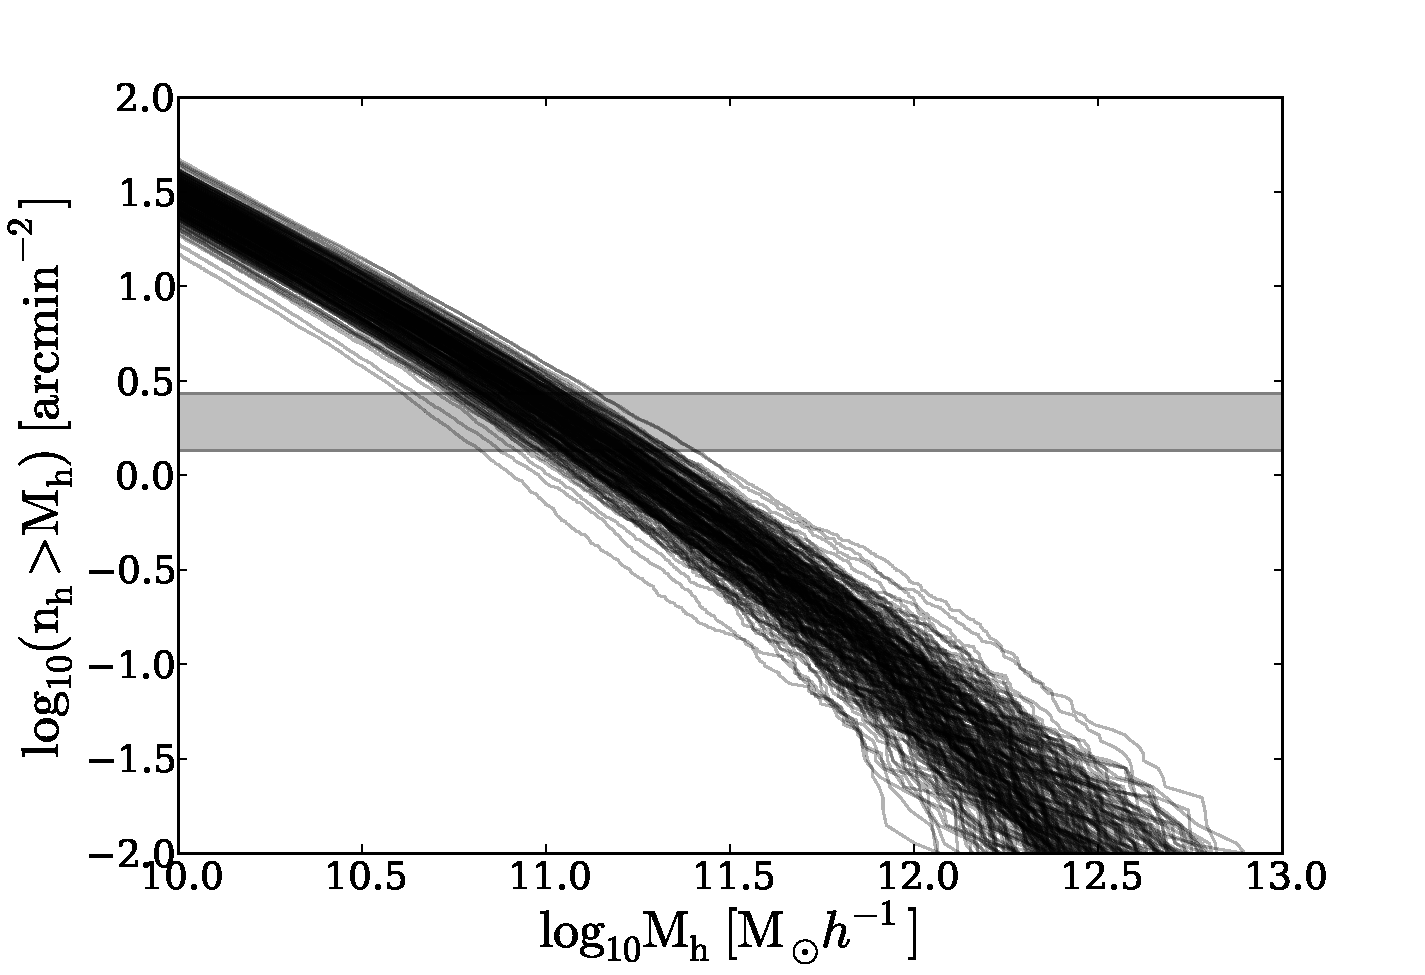
\includegraphics[width=1.10\linewidth,angle=0]{./plots/Fig1.pdf}
\caption{ \label{fig:halos} Surface density of dark
  matter halos as a function of a minimum halo mass to count the
  total number of elements in a volume. Each line represents on of the
  $210$ volumes of dimensions $46\times 35\times 41$ h${-3}$Mpc$^{3}$
  in the Bolshoi simulation. The horizontal gray band represents the
  range of surface densities observed for LAEs at $z=3.1$ as reported
  by \citep{Yamada2012}.}
\end{center} 
\end{figure}


\subsection{Dark Matter Halo Number Density}

In Figure \ref{fig:halos} we present the results for  the
integrated dark matter halo surface density as a function of halo
mass. Each line corresponds to one of the 210 sub-volumes in the
Bolshoi simulation. The gray band indicates the surface density
values for LAEs allowed reported in observations \citep{Yamada2012}.
 
This result provides the basis to understand why only a specific range of models
${\mathcal M}$ can be expected to be consistent with
observations. From Figure \ref{fig:halos} we can read that models
with a minimum mass $\log_{10} M_{\rm min}>11.5$\hMsun \ will always have a
surface number density lower than the observational
constrain. This makes impossible that models with that minimum mass
can be compatible with observations.


The opposite is true in models with $\log_{10} M_{\rm min}<10.5$
that will show surface number density larger than observations, this
implies that in such models the occupation fraction has to be tuned
$f_{\rm occ}<1.0$ as to lower the halo number density to match the
gray band values.

In the next subsection we quantify this intuition by means of the
Kolmogorov-Smirnov tests between mock surveys and observations. 

\subsection{Three halo mass ranges}

\begin{figure*}
\begin{center}
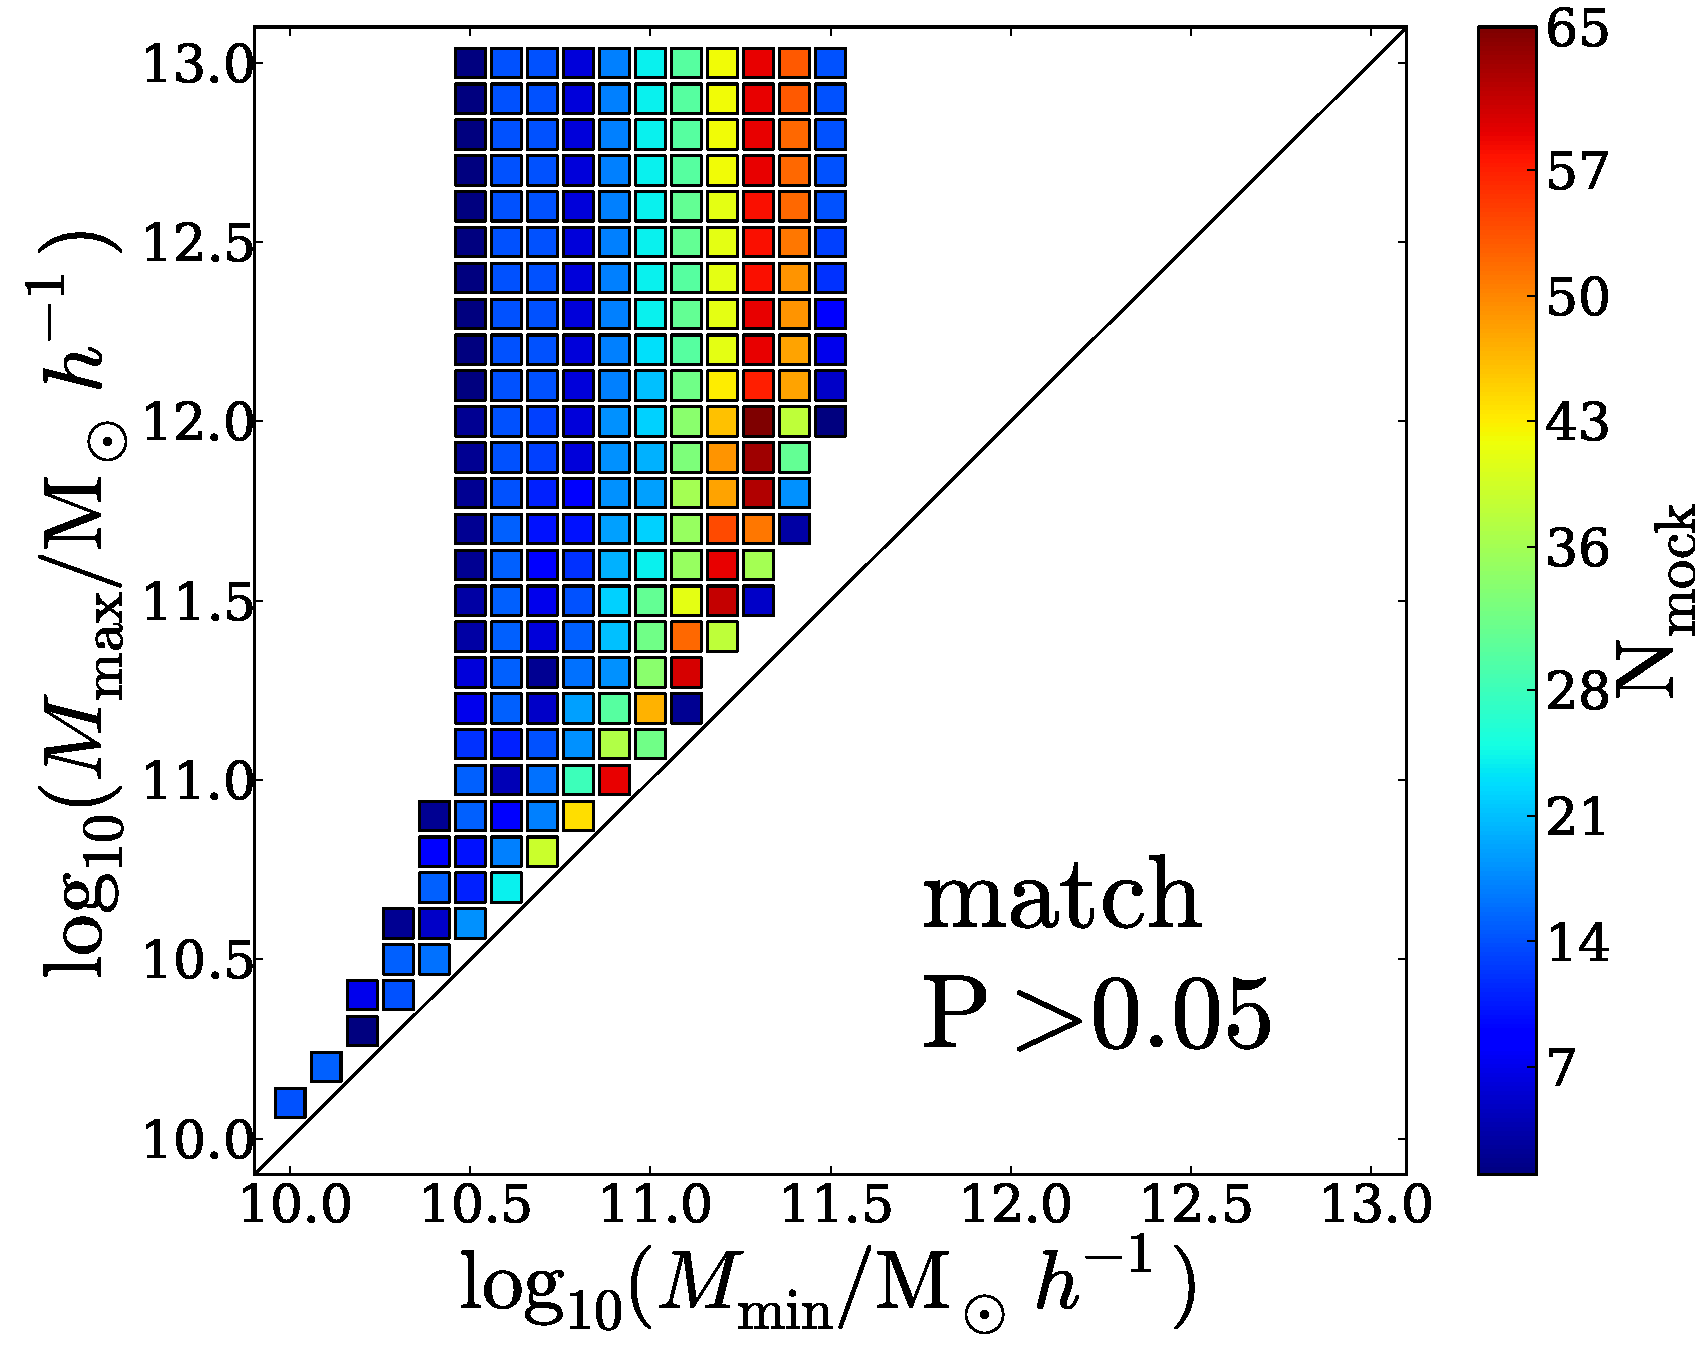
\includegraphics[width=0.46\linewidth,angle=0]{./plots/Fig2_match_P5.pdf}
\vspace{5mm}
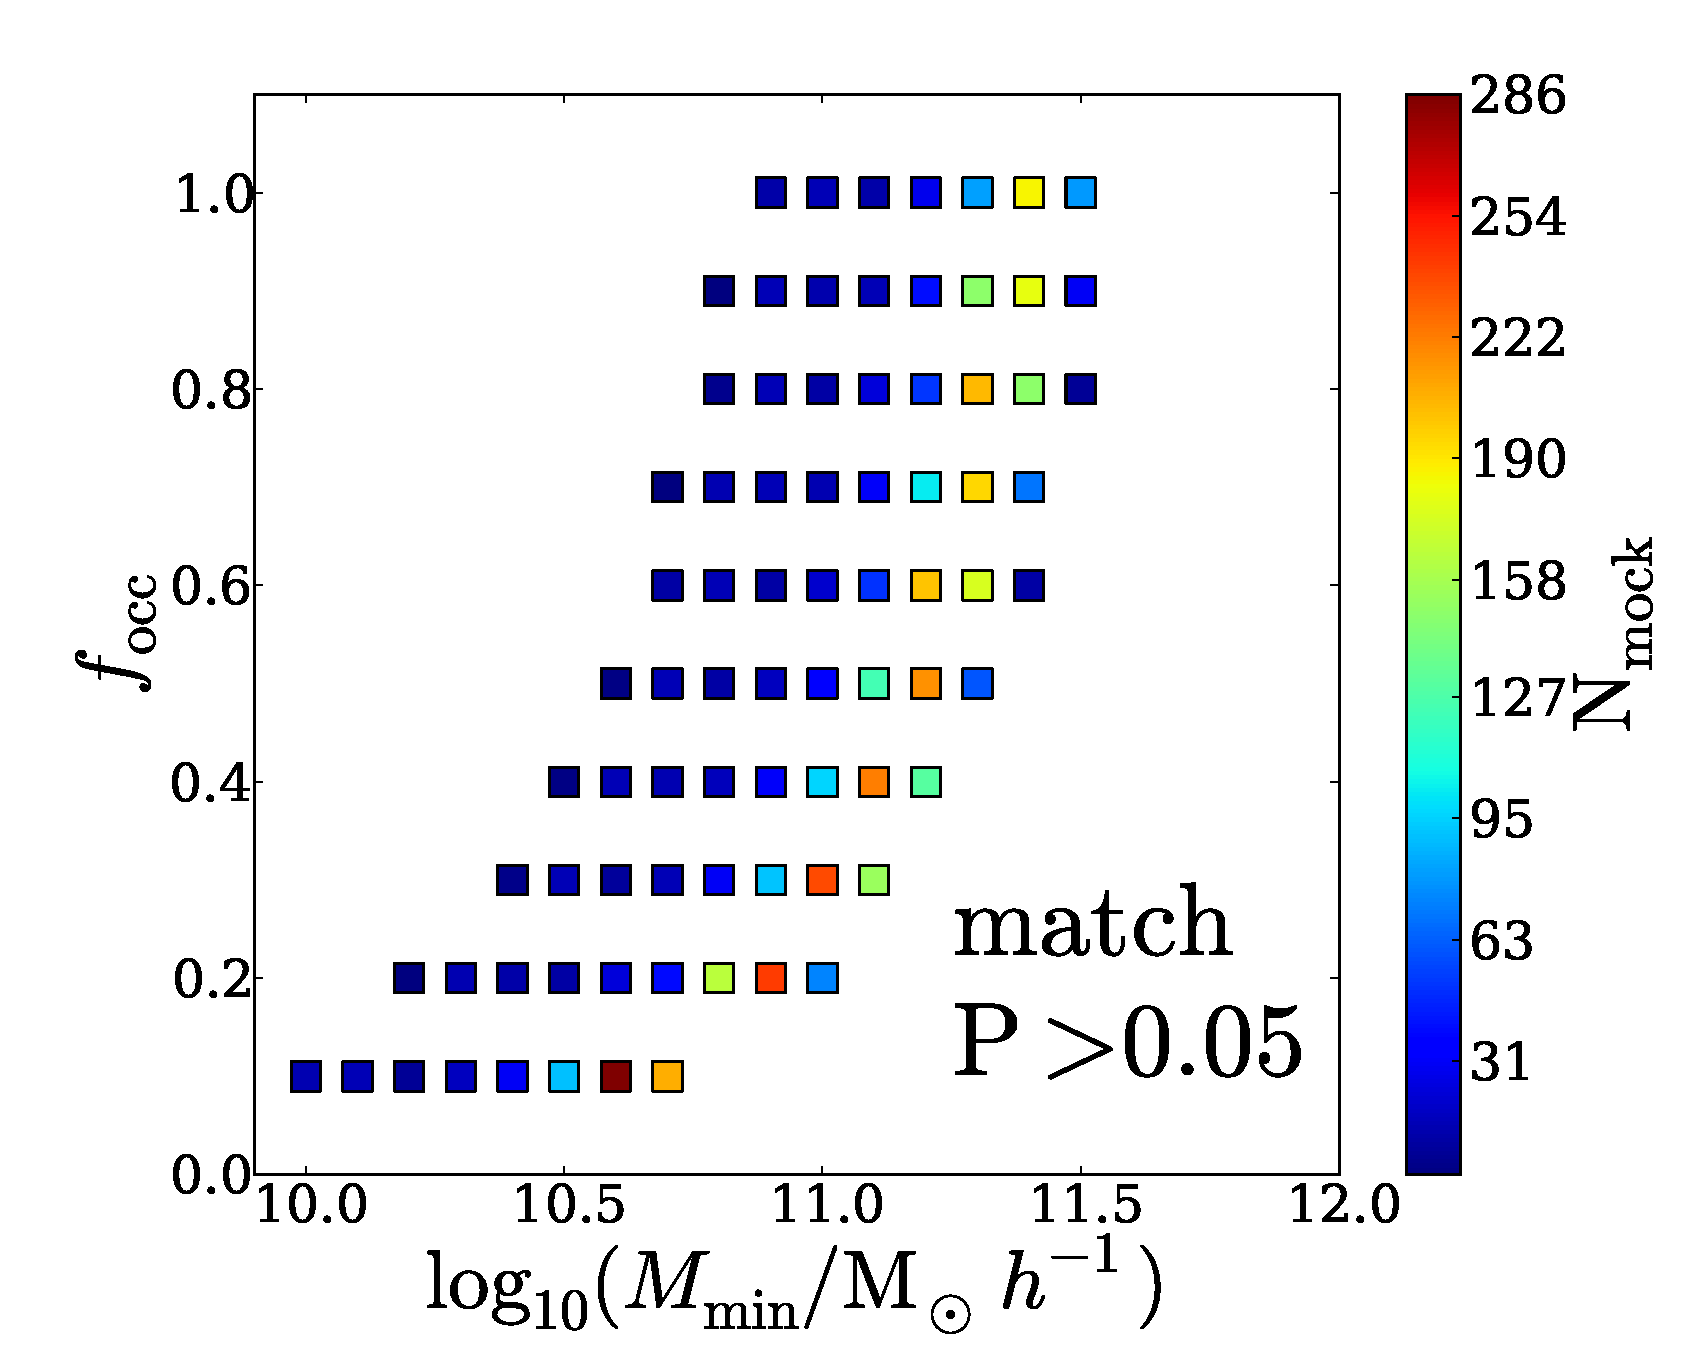
\includegraphics[width=0.49\linewidth,angle=0]{./plots/Fig3_match_P5.pdf}\\
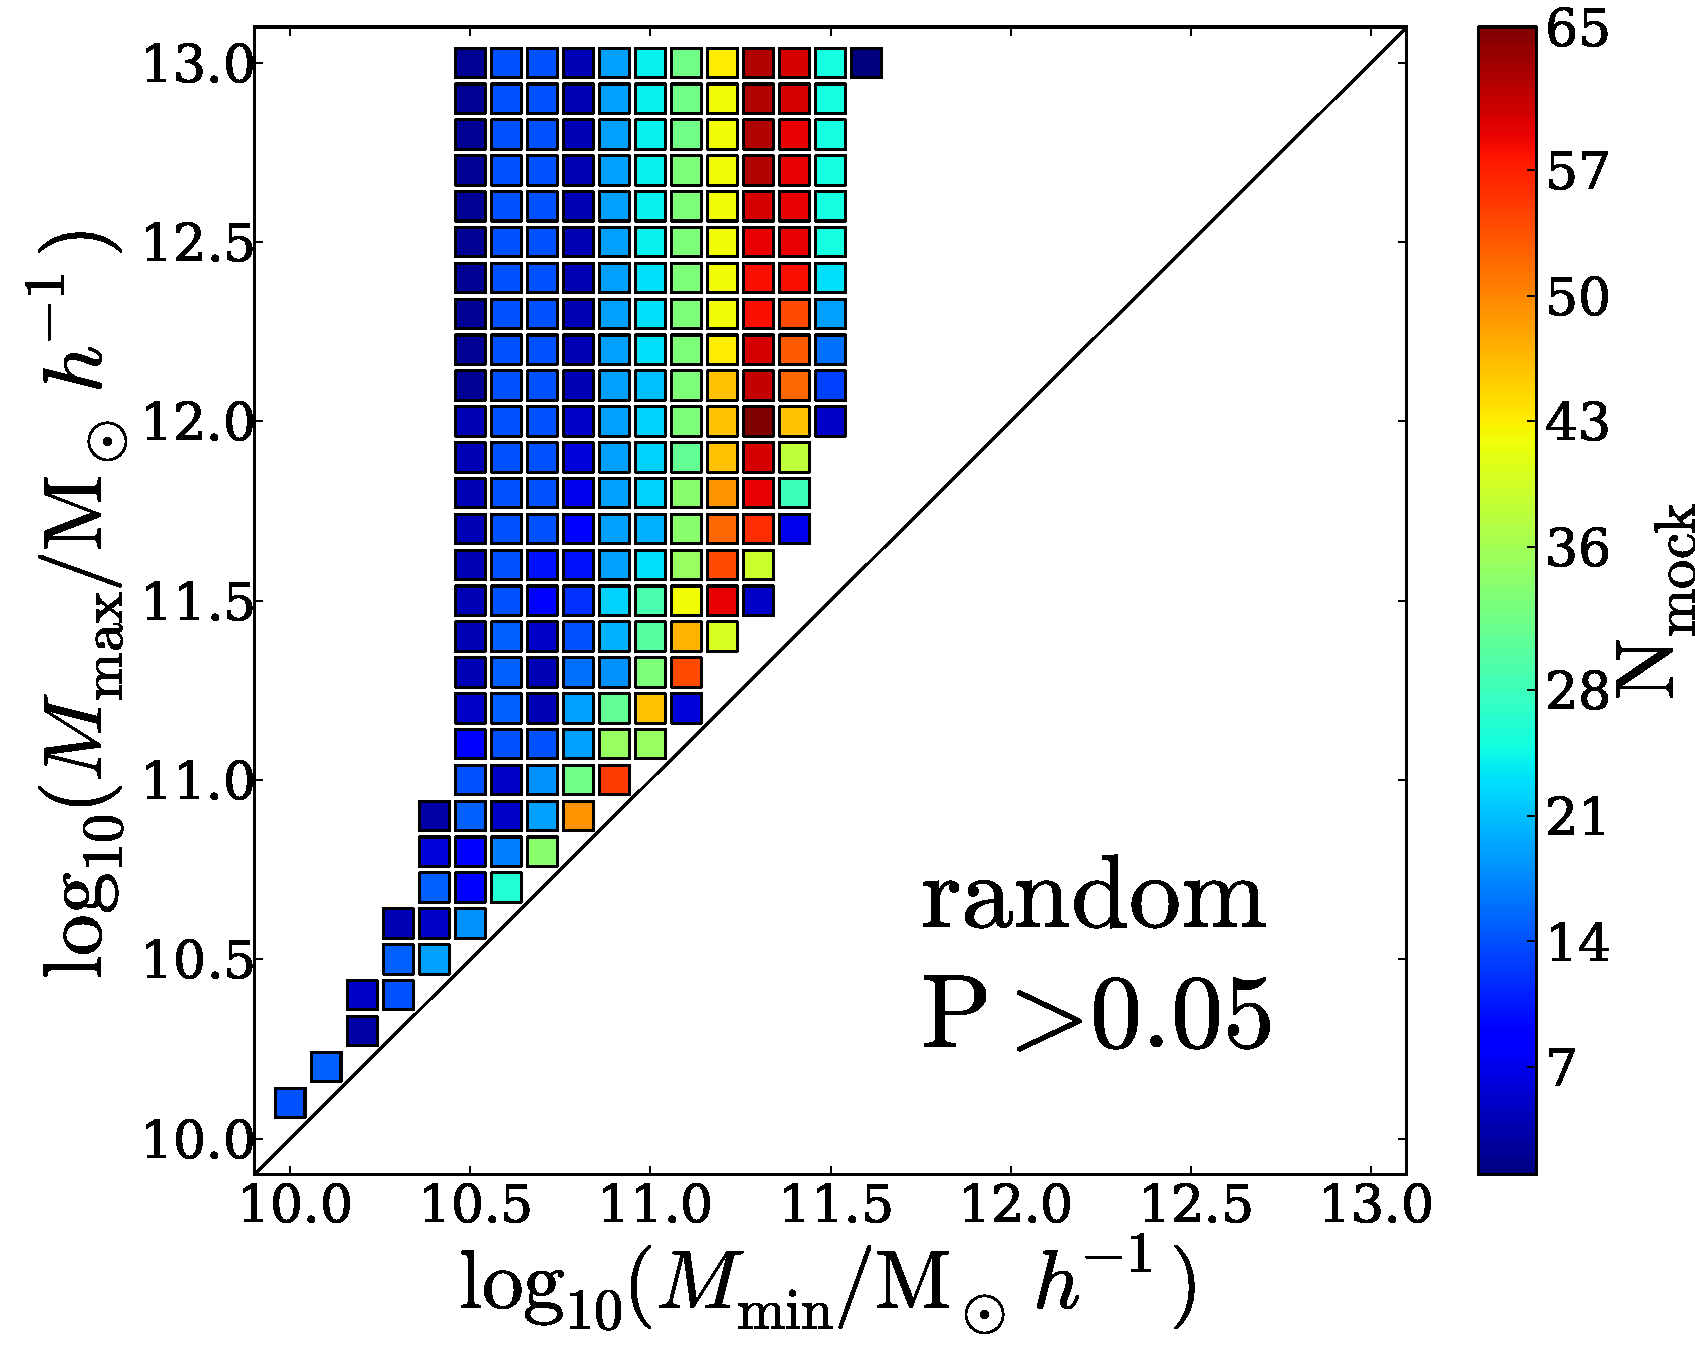
\includegraphics[width=0.46\linewidth,angle=0]{./plots/Fig2_random_P5.pdf}
\hspace{5mm}
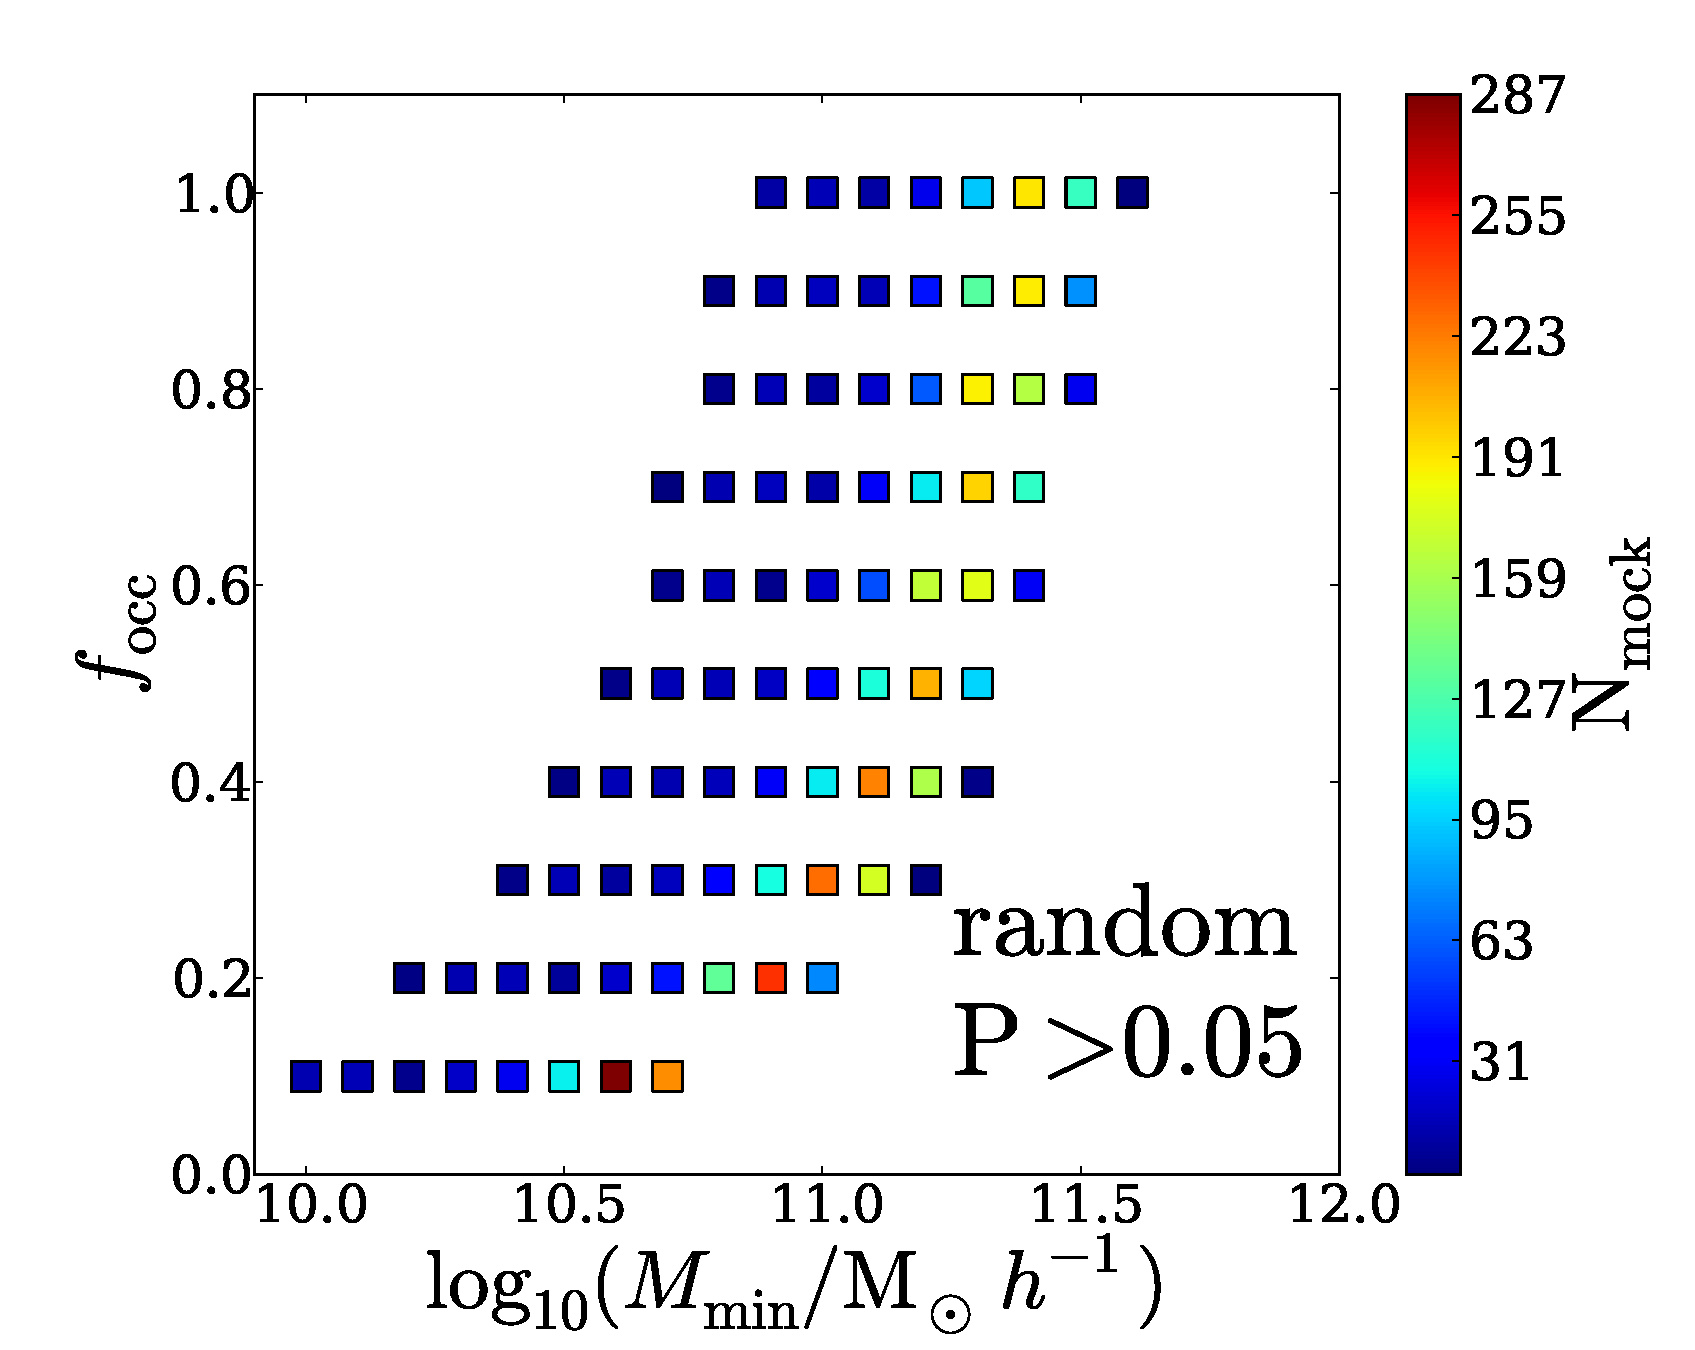
\includegraphics[width=0.49\linewidth,angle=0]{./plots/Fig3_random_P5.pdf}\\
\end{center} 
\caption{$M_{\rm min}$-$M_{\rm max}$ (left) and $M_{\rm
    min}-f_{\rm occ}$ (right) planes for all models with
  $P>0.05$ in two different ways used to construct the mock
  surveys. The color code corresponds to the number of mock surveys
  that are found to be compatible with observations in terms of the KS
  test with $P>0.05$. Only regions of parameter space with at least
  one (1) consistent mock survey are included. \label{fig:landscape}}   
\end{figure*}


Figure \ref{fig:landscape} presents regions in parameter space $M_{\rm
min}-M_{\rm max}$, $M_{\rm min}-f_{\rm occ}$ where the KS test yields
values of $P>0.05$ at least for one mock survey. For those models it
is not possible reject the hypothesis that the simulated and observed
data for the surface number density come from the same parent
distribution.

The upper (lower) panels correspond to the {\texttt match} ({\texttt
  random}) method to build the mock surveys from individual
fields. The plot shows number of mock surveys consistent
with observations. There are between $550$ to $600$ models out of the
original $9000$ models that have at least one (1) mock survey
consistent with observations. 


In Figure \ref{fig:landscape} there are three regions of parameter
space that can be clearly distinguished. The first region corresponds
to models where the minimum mass is high $\log_{10}M_{\rm min}>
11.5$. None of this models is compatible with observations as expected
from the results in the previous subsection. For these models the number
density of LAEs is too low compared to observations.

The second region corresponds to an intermediate range for the minimum
mass $10.5<\log_{10}M_{\rm min}<11.5$ where regardless of the value of
the maximum mass $M_{\rm max}$ it is possible to tune the occupation
fraction $f_{\rm occ}$ to bring some of the mock observations into
good agreement with observations. In this region in parameter space
one can thus find two extreme kinds of models.  One kind where the
mass interval is very narrow with sizes smaller than $<0.3$ dex (a
factor of two in mass) and others where the mass interval is 
extended, larger than $1.0$ dex, going up to the maximum halo mass
present in the simulation at that redshift. 

The third region in parameter space corresponds to $\log_{10}M_{\rm
  min}<10.5$. In this case only models with a very narrow mass interval of
at most $0.5$ dex ($\log_{10}M_{\rm max}<11.0$) and low
occupation fractions $f_{\rm occ}<0.3$ are allowed. 

Without any additional information our method allows us to infer that
most of the successful models are found in the second and third region of
parameter space where. This result was already expected from halo
abundance calculations shown in Figure \ref{fig:halos}. In the next
section we reduce the size of this region by imposing tighter
constraints on the KS tests and consistency with the angular
correlation function.

\begin{figure*}
\begin{center}
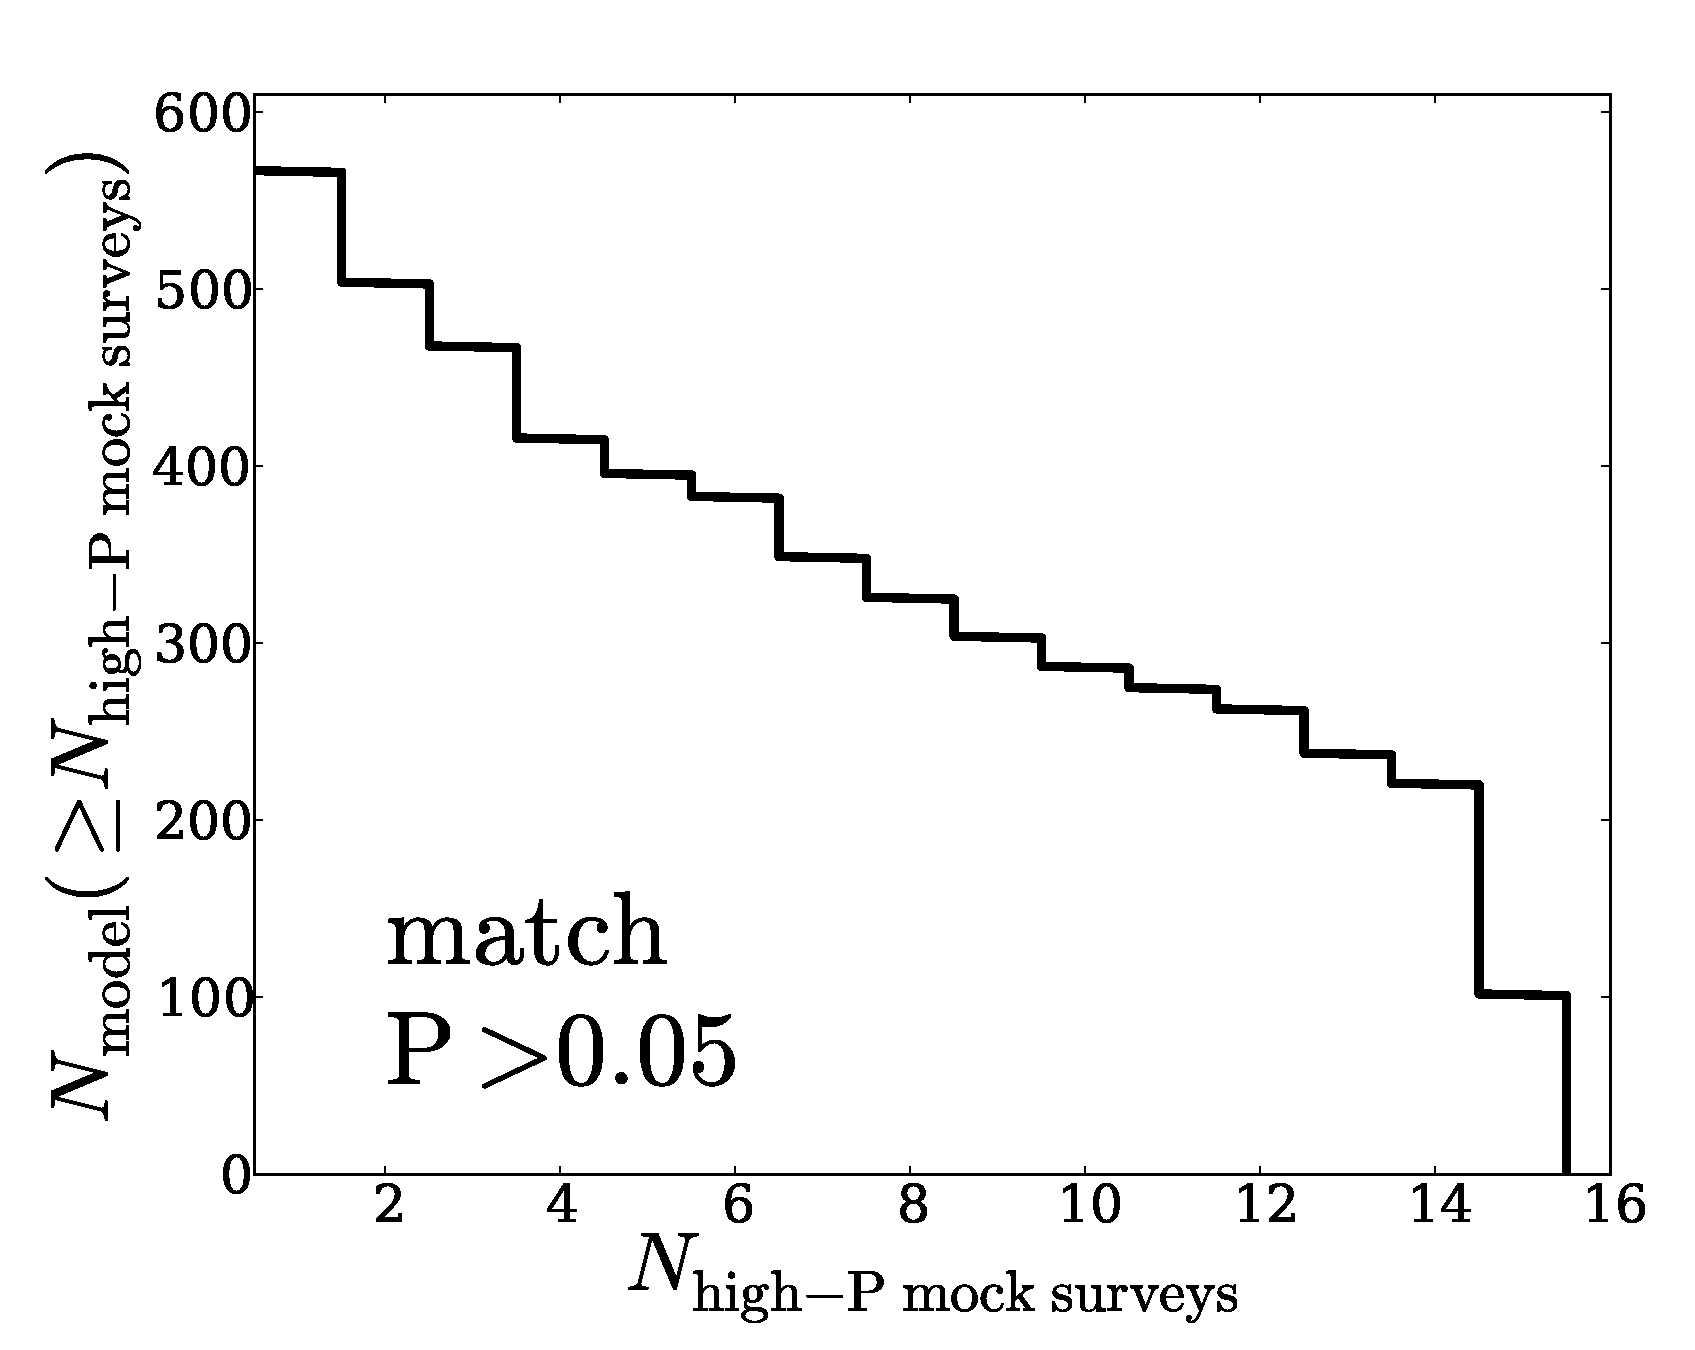
\includegraphics[width=0.46\linewidth,angle=0]{./plots/Fig4_match_P5.pdf}
\hspace{5mm}
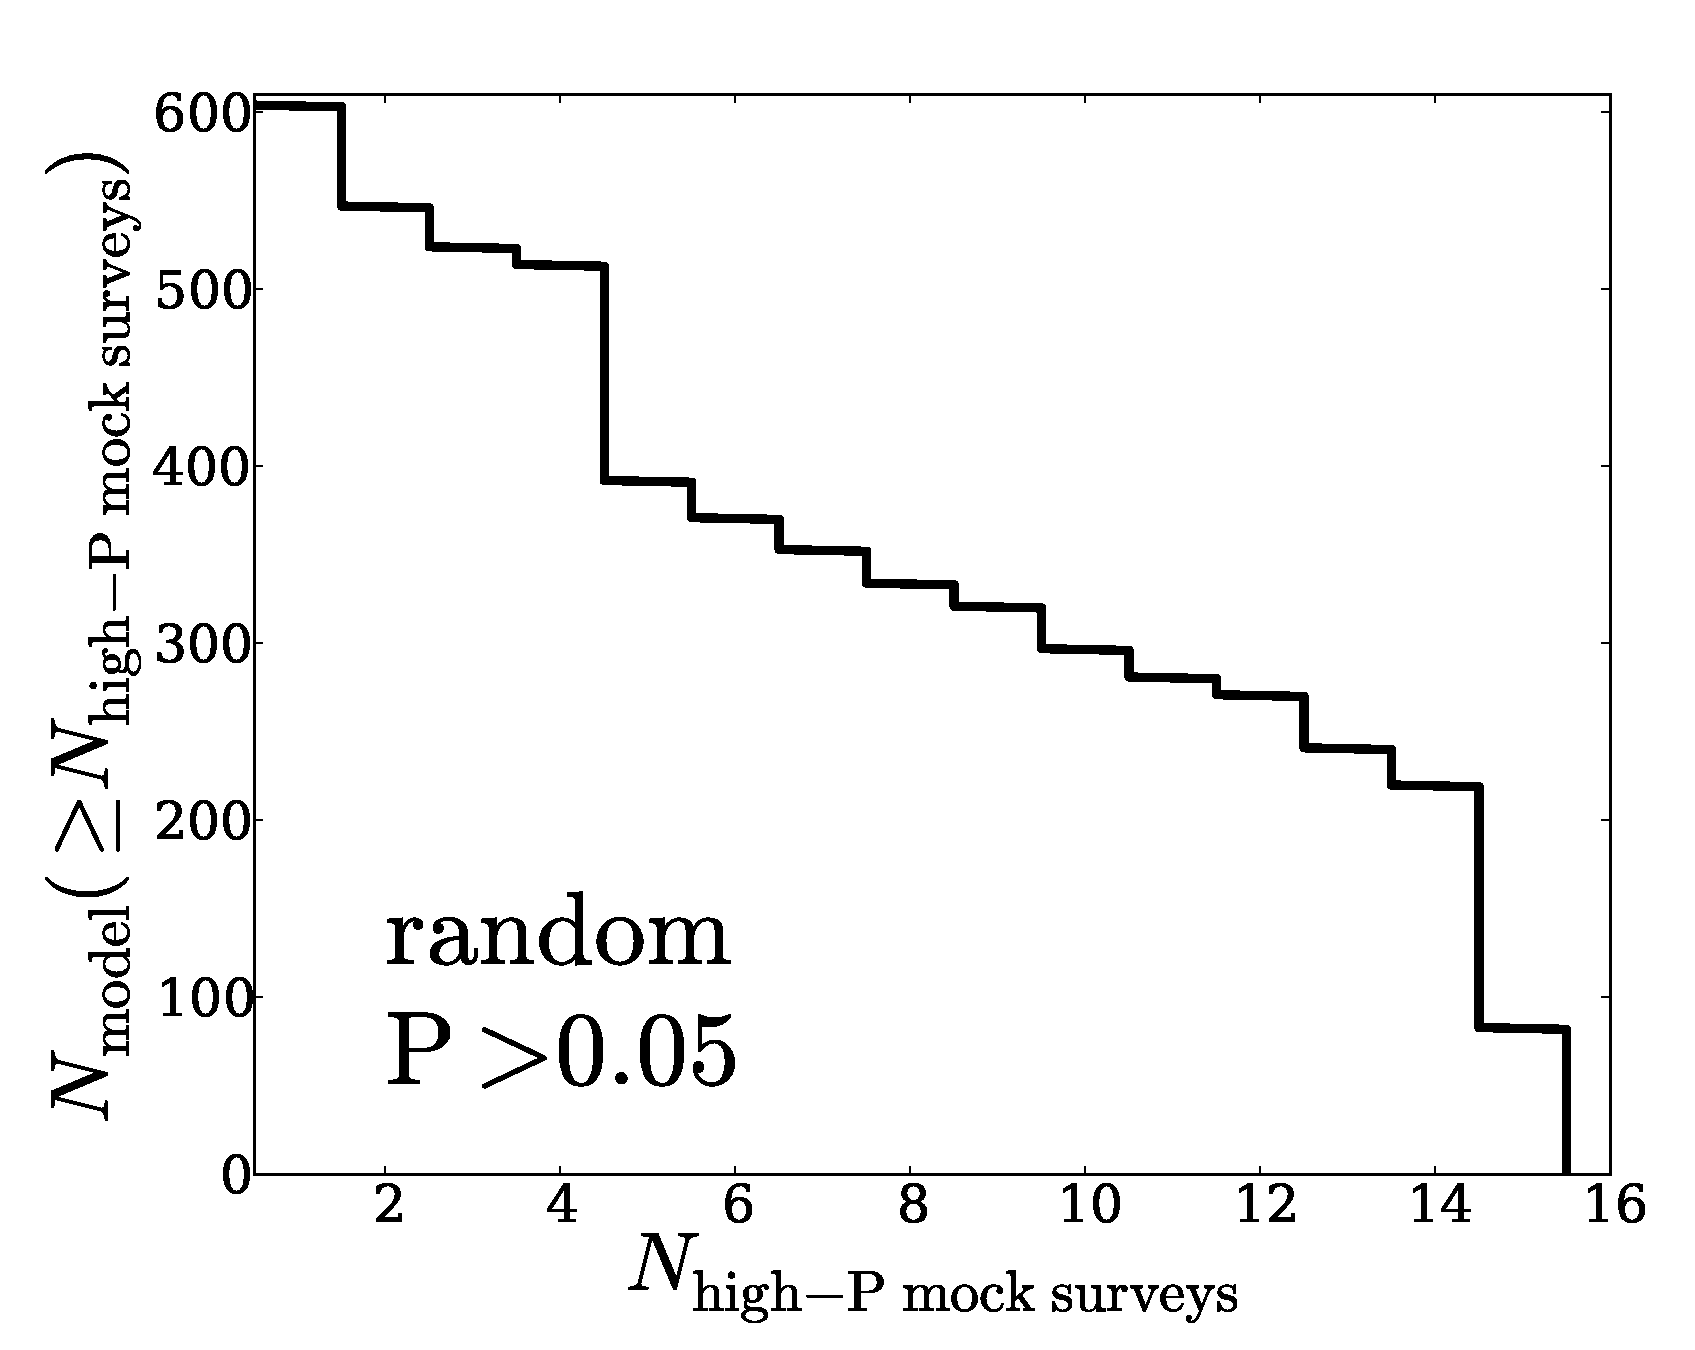
\includegraphics[width=0.46\linewidth,angle=0]{./plots/Fig4_random_P5.pdf}
\end{center} 
\caption{ Number of models with a minimum number of mock survey
  realizations that are consistent with observations.
  \label{fig:high_success_rate}.}  
\end{figure*}
 
\subsection{Models with the highest success rates}

For each model ${\mathcal M}$ there are 15 different mock surveys. In the
previous section we presented the models that had at least one (1)
mock survey with $P>0.05$.

Figure \ref{fig:high_success_rate} shows the number of models
that have at least $N_{\rm high-P}$ mocks with $P>0.05$ for both the
{\texttt  match} and {\texttt random} methods.  This shows that there
are between $80$ to $100$ models with all the 15 realizations with
$P>0.05$. Selection of these models as successful represents a
reduction of a factor of $\sim 6$ with respect to the total number of
mocks with at least one consistent mock.  

Figure \ref{fig:restriction_mock} presents the locii of these models
in the parameter space $M_{\rm min}-M_{\rm max}$ and $M_{\rm
  min}-f_{\rm occ}$. The results are very similar between the {\texttt
  match} and {\texttt random} methods. With this constraints the
number of consistent models with  $\log_{10}M_{\rm min}< 11.5$ are
greatly reduced. This corresponds to the regions in the parameter
space in Figure \ref{fig:landscape} that already had a low number of
consistent mock surveys. On the other hand, from the right panel in
Figure \ref{fig:restriction_mock} one can see that there is not a
strong selection effect on the occupation fraction $f_{\rm occ}$.  


\begin{figure*}
\begin{center}
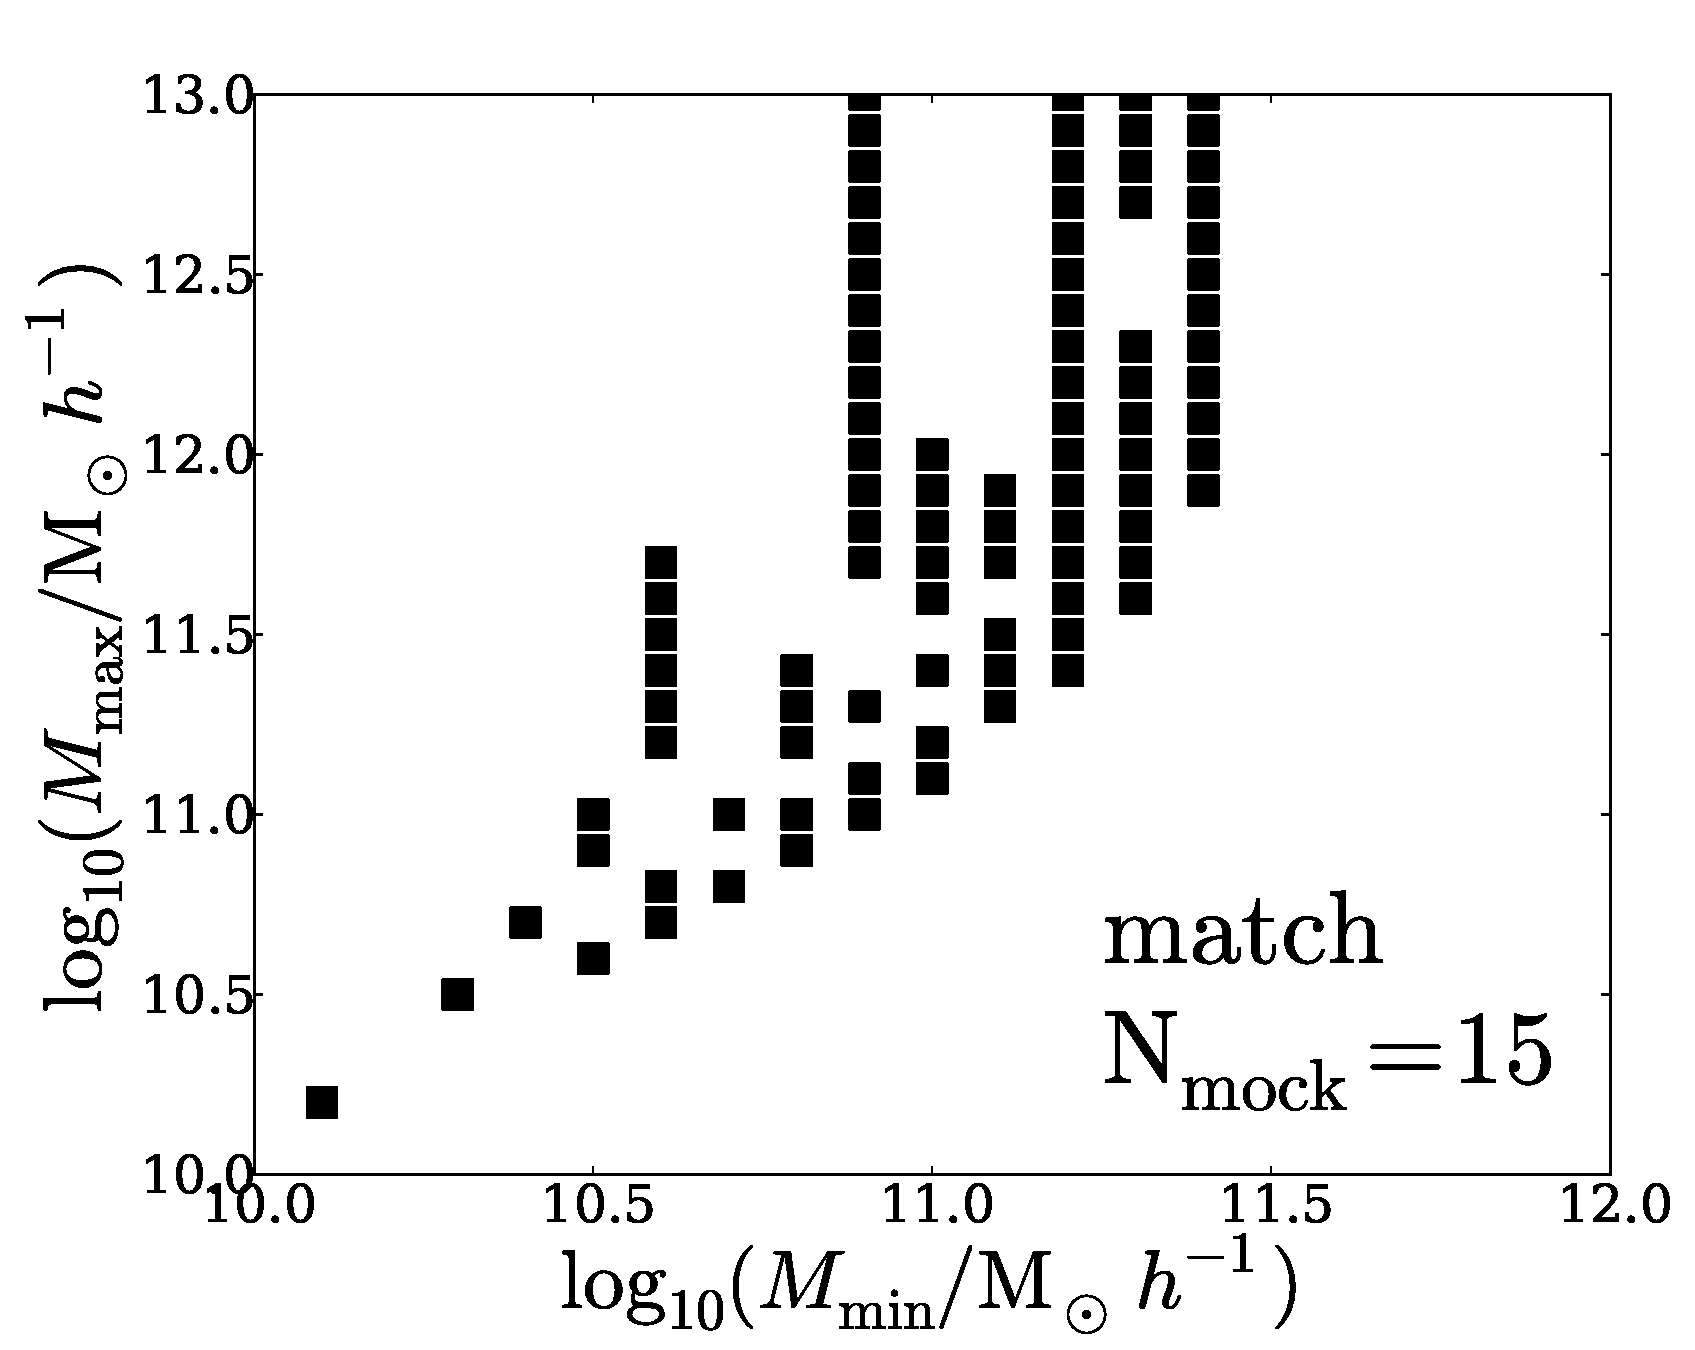
\includegraphics[width=0.46\linewidth,angle=0]{./plots/Fig5_match_mass_mock.pdf} 
\hspace{5mm}
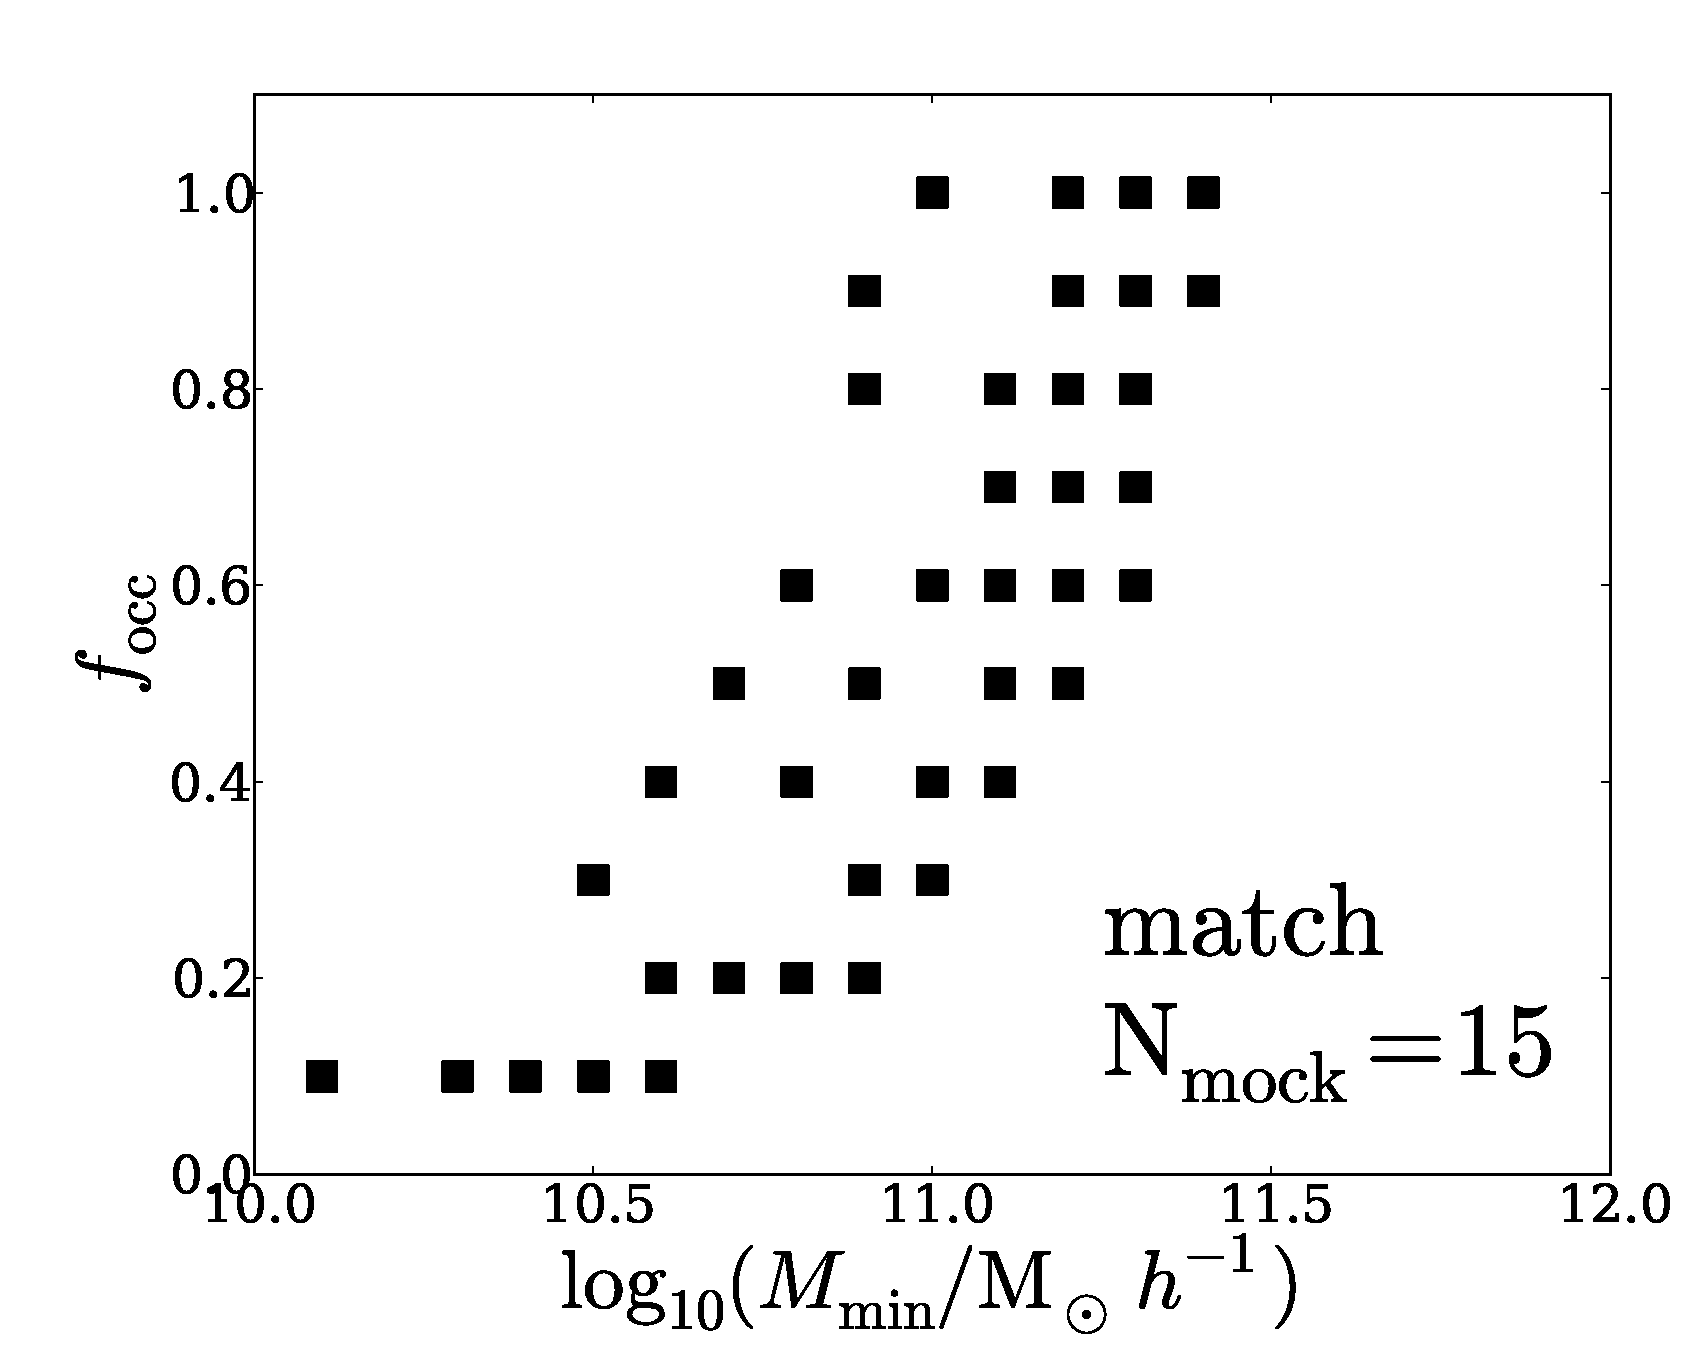
\includegraphics[width=0.46\linewidth,angle=0]{./plots/Fig5_match_f_occ_mock.pdf}
\end{center}  
\caption{Favored regions in parameter space when the constraints on
  the maximal number of consistent mocks is imposed. The results for
  the {\texttt random} methodology (not shown here) are very similar to the ones
  presented here for the {\texttt match} method.
  \label{fig:restriction_mock}}  
\end{figure*}



\subsection{Consistency with the Angular Correlation Function}



\begin{figure*}
\begin{center}
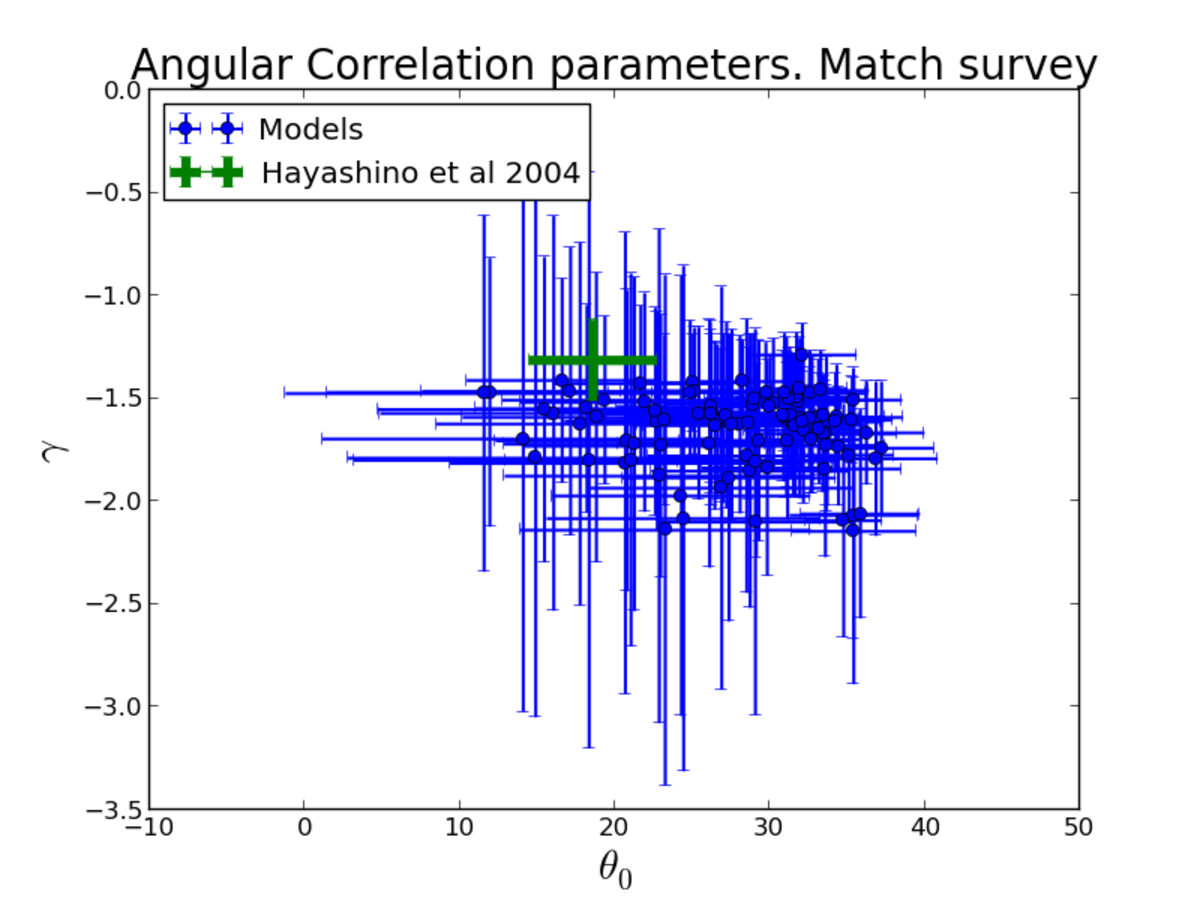
\includegraphics[width=0.46\linewidth,angle=0]{./plots/power_law_correlation.pdf} 
\hspace{5mm}  
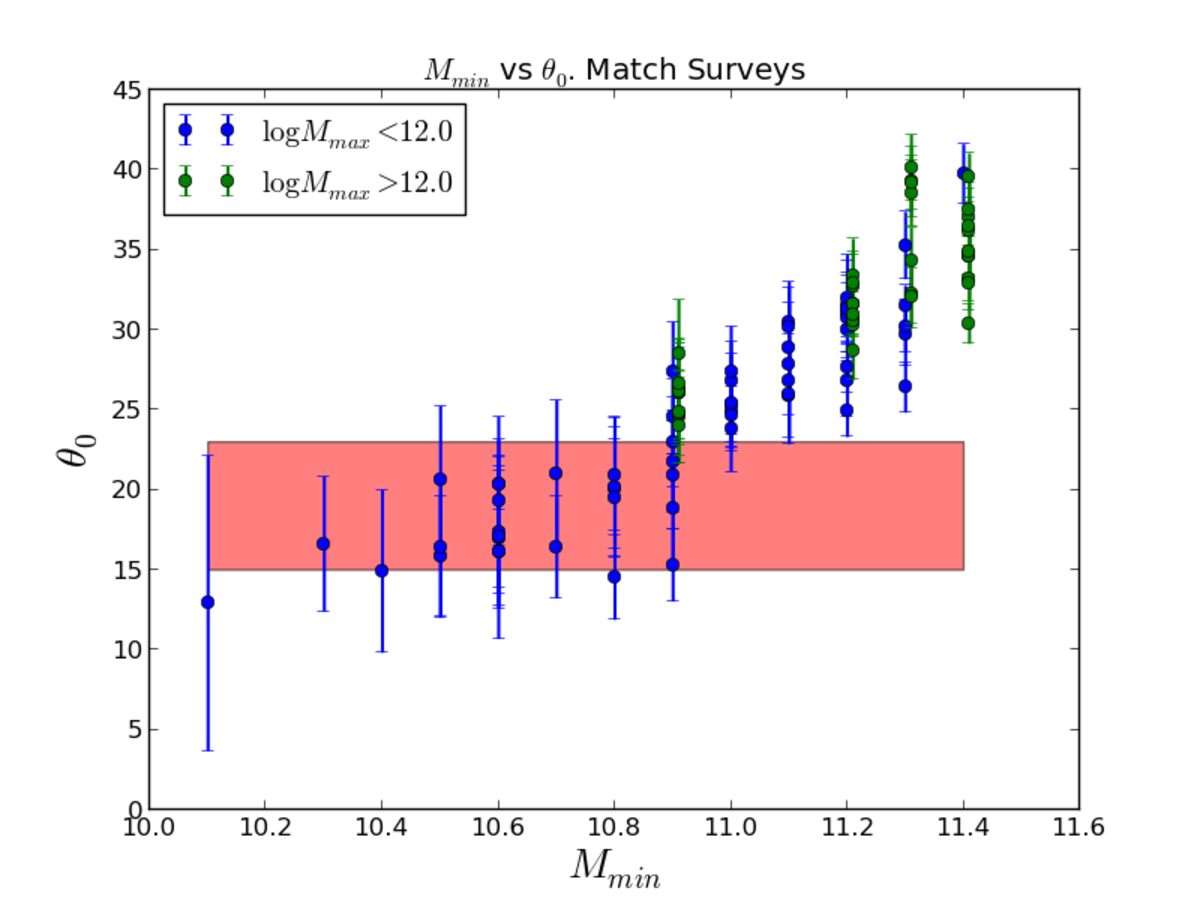
\includegraphics[width=0.46\linewidth,angle=0]{./plots/mmin_vs_correlation.pdf} 
\end{center}
\caption{Left: Values for the free parameters ($\theta_{0}$ vs $\gamma$) 
in the fitting formula (Eq. \ref{eq:fitting}) for the mean angular
correlation function. Blue dots correspond to simulations and the green cross to
observations by \citet{Hayashino2004}. The error bars in the 
theoretical data correspond to the standard deviation from the
different mocks surveys. Right: Same results as before in the shown in
the $\theta_{0}$-$M_{\rm min}$ plane. This time the observational
constraints are represented by the red rectangle. Blue squares
represent models with $\log_{10} M_{\rm  max}<12.0$, green circles
correspond to models with $\log_{10} M_{\rm max}>12.0$. 
\label{figure:correlation_parameters}}
\end{figure*} 


\begin{figure*}
\begin{center}
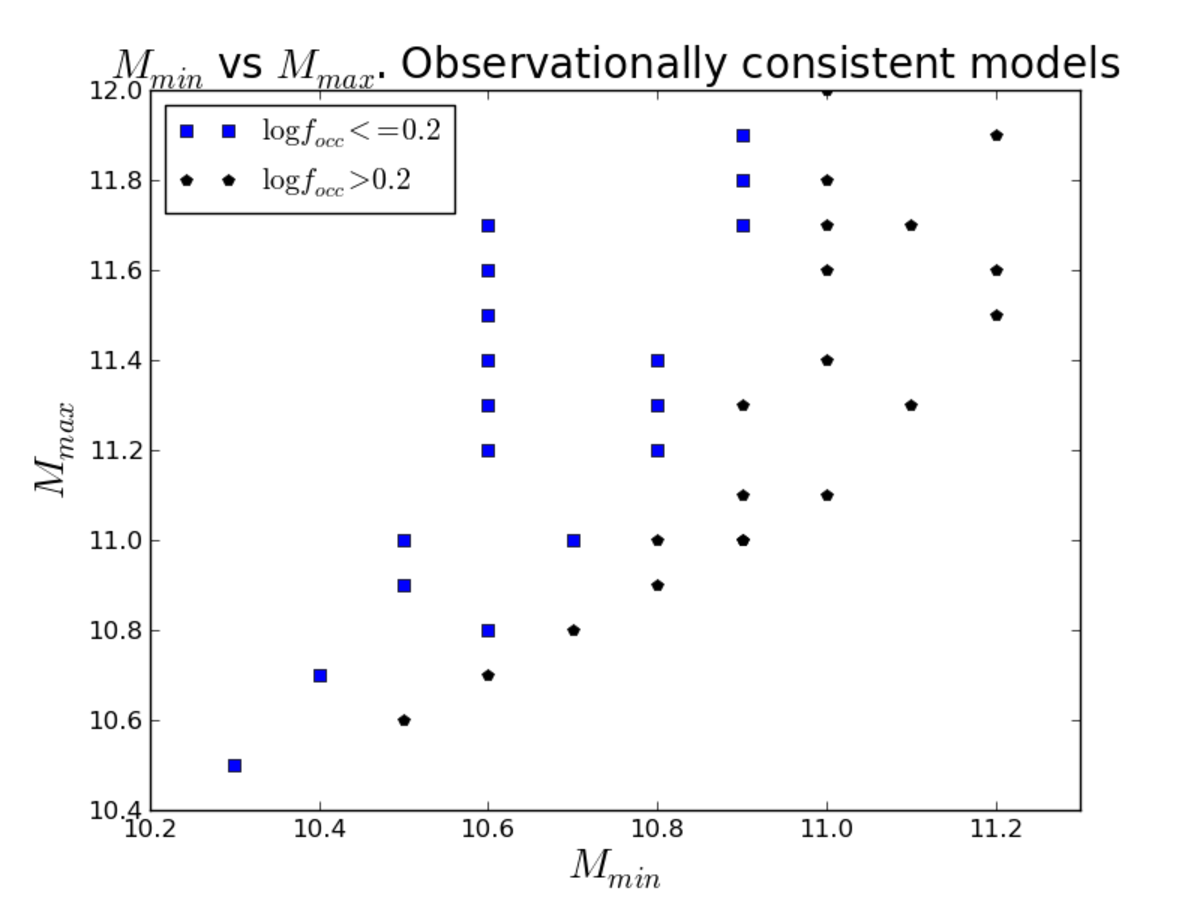
\includegraphics[width=0.46\linewidth,angle=0]{./plots/mmin_vs_mmax.pdf}
\hspace{5mm}
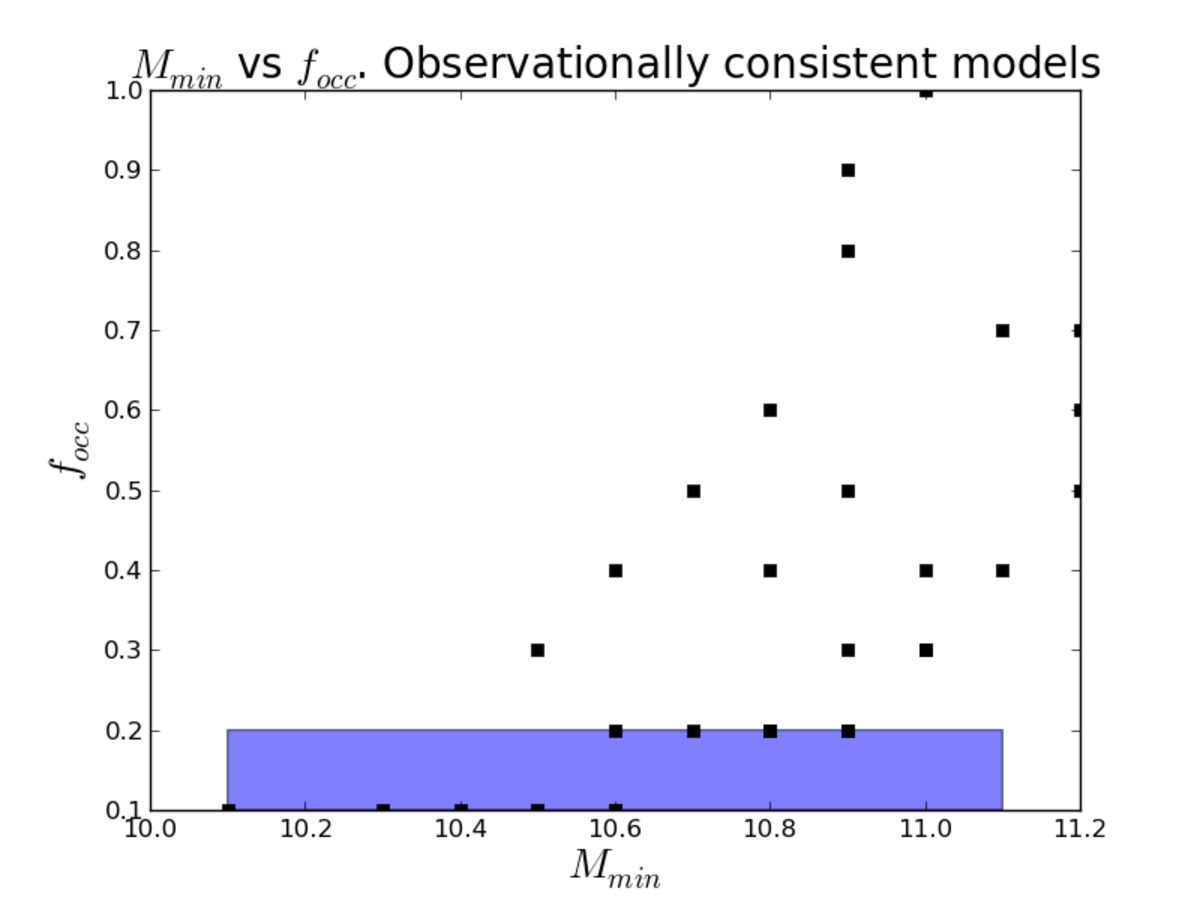
\includegraphics[width=0.46\linewidth,angle=0]{./plots/mmin_vs_focc.pdf}
\end{center}
\caption{Best models parameter space when both the constraints on the
  maximal number of  consistent mocks and the occupation  fraction
  $f_{\rm occ}\leq  0.2$ are included. $M_{\rm min}$ vs $M_{\rm max}$
  (left), $M_{\rm min}$ vs $f_{\rm occ}$ (rigth).
  \label{fig:restriction_mock_and_f_occ_corr}} 
\end{figure*} 


Figure \ref{figure:correlation_parameters} shows the main results in a
$\theta_{0}-\gamma$  plane where the average and standard deviation
for each mock is shown in comparison with the result derived from
observations.  The error bars in this Figure represents the standard
deviation of the ACF over all the sub-fields in the 15 mock
observations. These error bars are larger than the statistical
uncertainty from the fitting procedure on a single field.

In the left panel Figure \ref{figure:correlation_parameters} we see how
the observational ACF measured by \cite{Hayashino2004} (green dot) is
successful in reducing the total number of possible models. Only those
with angular-correlation length within
$15^{\prime\prime}<\theta_{0}<23^{\prime\prime}$ are considered to
reproduce observations.    


In order to better illustrate the results from this test we
show in the right panel of Figure \ref{figure:correlation_parameters} 
the plane $\theta_{0}$-$M_{\rm min}$ for all models. There we divide
the models into two disjoint sets: those with $\log_{10} M_{\rm
    max}<12$ (blue dots) and $\log_{10} M_{\rm
    max}>12$ (green dots). The colored rectangle includes
the parameter region which is consistent with the observational
constraint in $\theta_{0}$. With this restriction we find that most
models with $\log_{10} M_{\rm max}>12$ and  $\log_{10} M_{\rm min}>11.1$ 
%can be safely ruled out.  



In Figure \ref{fig:restriction_mock_and_f_occ_corr} we present the preferred
models in the planes $M_{\rm min}-M_{\rm  max}$ and $M_{\rm min}-f_{\rm occ}$
for the {\tt match} method after applying the observational constraints 
in the occupation fraction and the ACF. Here we consider a model
consistent if there is an overlap of $1-sigma$ in its values for the
correlation length $\theta_0$ and the power $\gamma$ in the
correlation function.  


\section{Discussion}

Matching the galaxy surface number density statistics sets the median
mass of all successful models in the range $10^{10}-10^{12}$
\hMsun. Including more strict criteria on the number of mock surveys
that must be consistent with those observations and additional
information from the angular correlation function greatly reduces the
number of possible models. We end up with $\sim 50$ models out of the
initial 90000 possible combination of parameters.  

We find that to make a physical interpretation of these models it is
useful to do it in terms of the size of halo mass range. We now use the
variable $\Delta M=\log_{10}M_{\rm max} - \log_{10}M_{\rm  min}$, together
with the escape fraction $f_{\rm occ}$ to help us build a classification
of all the successful models into three families: 


\begin{itemize}
\item[(1)] Low $f_{\rm occ}\leq 0.3$ and low $\Delta M\leq 1.0$
  dex: 24 models.
\item[(2)] Low $f_{\rm occ}\leq 0.3$ and high $\Delta M > 1.0$dex: 11
  models
\item[(3)] High $f_{\rm occ}> 0.3$ and low $\Delta M\leq 1.0$: 14 models
\end{itemize}

There is a clear majority of models with a narrow $\Delta M\leq
1$, compared to the $2.5$dex of halo mass available for occupation at
that redshift. Such models imply that there is a cut at lower and higher halo
masses that render inefficient the presence and/or detection of LAEs.

At the low mass end, such cut can be readily interpreted in terms of the
minimal halo star formation rate needed to produce the necessary \lya
luminosity to be above a given detection threshold.  However, under
the reasonable assumption of star formation rate increasing with halo
mass, the cut at higher halo masses requires a different explanation. 

One possible interpretation can be made in terms of a decreasing escape
fraction of \ly radiation in massive systems. There are detailed models for
radiative transfer that support the idea that massive galaxies with
higher metallicities have larger dust contents than lower mass
systems, which due to the resonant nature of the \ly line are enough
to produce high absorption of \ly photons but not of continuum or
other non-resonant lines.  

The preference for narrow $\Delta M$ ranges to hosting LAEs together
with the total absence of reasonable models with $M_{\rm max}>
10^{12}$\hMsun \  shows that our models support theoretical insights
where the most massive systems are not bright \ly sources
\citep{ForeroRomero2012}.   

\subsection{Comparison against results from blind surveys}

We also find that $70\%$ of the best models are found in families (1)
and (2), with a low occupation fraction $f_{\rm occ}\leq 0.3$. This
preference goes in the same direction as the observational constraint
on $f_{\rm occ}\sim 0.1-0.2$ derived at $z=2.2$ by \cite{Hayes2010}
and recent theoretical study of observational data in a wide redshift
range $0<z<6$  \citep{Dijkstra2013}. 

The observational estimation by \cite{Hayes2010} was based on blind
surveys of the H$\alpha$ and Lyman $\alpha$ line. Using corrections by
extinction to obtain an estimate for the intrinsic H$\alpha$
luminosity, and using values for the theoretical expectation of the
ratio Lyman$\alpha$/H$\alpha$ they derive an bulk escape fraction for
the Lyman$\alpha$ radiation of $f_{\rm esc}=(5.3\pm 3.8)\%$ or $f_{\rm
  esc}=(10.7\pm 2.8)\%$ if a different dust correction is used. 

They also showed that that the luminosity function for LAEs at $z=2.2$ is
consistent with the escape fraction being constant for every galaxy
regardless of its luminosity. From this results they derive that
almost $90\%$ of the star forming galaxies emit insufficient
Lyman $\alpha$ to be detected, effectively setting the occupation
fraction to be $f_{\rm occ}=0.10$.  

\cite{Dijkstra2013} used a similar principle to derive their results. They
compared observationally derived star formation functions to LAE
luminosity functions. At $z\sim 3.0$ they derive an effective escape
fraction of $f_{\rm esc}=(17\pm 5)\%$ could be interpreted as an
occupation fraction $f_{\rm occ}\sim 0.2$.  We consider a success of
our method the fact that we find that most of the consistent models
show a low occupation fraction.    



\subsection{Comparison to other clustering estimates}

Observational based on the ACF inferred from photometric measurements
in the Extended Chandra Deep Field South have shown that the median
dark matter masses of h los hosting LAEs is $\log_{10}M_{\rm
  med}=10.9^{+0.5}_{-0.9}$\Msun, with a corresponding occupation
fraction of $1-10\%$  \citep{Gawiser07}.  Our results are in a general
good agreement with those estimates for the host mass. This is not
completely unexpected given that we have also required consistency
with ACF measurements.   

The novelty in our approach is that we have a detailed estimate for 
host halo mass range together with the escape fraction. This allows us
to demonstrate that the halo mass range could be very narrow $\Delta M <
0.2$dex, something that cannot be inferred from ACF analysis
alone. 

We also find interesting that our ACF analysis is also not enough to rule
out models with a high occupation fraction $f_{\rm occ}>0.3$, which
represent almost one fourth of our best models, coinciding with a wide
range in halo masses $\Delta M>1.0$ dex. These models can only be
considered unfavorable based on a different set of observations as we
have described in the previous subsection.


\subsection{In the context of abundance matching models}


Considering the additional evidence for a low escape fraction we can
say that the preferred models are in families (1) and (2) with a
clear majority composed by those with narrow mass range and low occupation
fraction.  

Using abundance matching methods throughout cosmic time from redshifts
$0<z<8$ \cite{Behroozi2013a,Behroozi2013b} report that the instantaneous star
formation efficiency (star formation rate divided by the stellar mass)
presents a clear maximum around $10^{11.7}$\Msun \ at all redshifts
$z<4$.

This mass scale is strictly superior to the great majority of  $M_{\rm max}$
values allowed in the models with low escape fraction. Using the results published
in \cite{Behroozi2013a} we find that the typical stellar mass in halos
of $10^{11.4}$\hMsun \ is $(1.0\pm0.3)\times 10^{9.0}$ \hMsun, while
their star formation rate is in the range $0.6\pm 0.2$ Msun yr$^{-1}$.
This halo mass range around $10^{11.4}$ \hMsun \ is the lower bound of
what is computed in the abundance matching model in order to fit the
observational data for the stellar mass function based on the
observations of Lyman Break Galaxies. 

All the preferred models have a halo mass range with $M_{\rm
  min}<10^{11.4}$\hMsun. This suggests that a detailed and careful
study of the spectral and photometric properties of LAEs coupled to the kind of
analysis performed in this paper can be a guide in the study of the
properties of low mass dark matter halos at $z=3.1$, extending the
capabilities of abundance matching methods.


\subsection{On the reproducibility of our results}

... All the software to produce the results in this paper is publicly
available. 

... The raw catalogs can be obtained from the MultiDark database but
can also be obtained in the repository of this paper on github.

\section{Conclusions}
\label{sec:conclusions}

In this \documentname we constrain the preferred dark matter mass
and occupation fraction for halos hosting Lyman Alpha Emitters at
redshift $z=3.1$ in a $\Lambda$CDM cosmology. We use a method that
matches the cosmic variance of the surface 
density number of LAEs between mock and real observations and is also
consistent with observational estimates for the angular
correlation function. The mock catalogs are constructed using a 
model with three basic parameters: the halo mass range where LAEs can
be found, $M_{\rm   min}<M_{\rm h}<M_{\rm   max}$, and the fraction of
the halos in this range that are actually occupied, $f_{\rm occ}$. After
a thorough exploration of the parameter space we find that wide
variety of models are consistent with the observational constraints,
where only a minority has been considered so far in the
literature. Out of $9000$ initial combinations for the model
parameters we end up with $49$ successful arrangement of parameters.


The most important conclusion of this work is that available
observational information for the clustering properties of LAEs at
$z=3.1$ does not provide enough constraints to uniquely narrow the range of masses
and occupation fraction of dark matter halos hosting those galaxies. In our
model, the hosting halos can be split into three families depending the mass range
$\Delta M=\log_{10}M_{\rm max} - \log_{10}M_{\rm min}$ and the
occupation fraction $f_{\rm occ}$. The first family is narrow both in
$\Delta M$ and $f_{\rm occ}$, a second family is only narrow in
$\Delta M$ and the third is narrow in $f_{\rm occ}$ and broad in
$\Delta M$. 


All the halo mass ranges in the best models fall into the broad
range obtained in previous analysis \citep{Gawiser2007}. The
improvement of our method is being able to describe in high detail
all the possible models consistent with observations, including the
discovery of models previously overlooked like those with a high
occupation fraction $f_{\rm occ}>0.3$.
 

A central result in this exploration of parameter esp ace is the
existence of a large number of models with a very
narrow mass range $\Delta M< 0.1$ dex that are consistent in every
aspect with the spatial distribution of observed LAEs. In order to
have these characteristics it is required that halos around the mass
$M_{\rm max}$ for each model become inefficient in hosting detectable
galaxies. One way to achieve this is having LAEs with a decreasing \ly
escape fraction with increasing mass. 

All the models also present a range of masses where the halos are
below the mass scale of $10^{11.4}$\hMsun \  inferred as a lower
threshold for the LBGs used in halo abundance matching
studies. Detailed study of high-z LAES will have a positive impact on
our understanding of the connection of low mass halos to star forming
galaxies.

We foresee that the new observations with new instruments (such as MUSE,
Hyper SuprimeCam and HETDEX) covering larger fields and a wider range
of luminosities will be key in imposing tighter constraints on the
properties of dark matter halos hosting LAEs.  


\section*{Acknowledgments} 
J.E.F-R thanks the hospitality of Changbom Park and the Korea
Institute for Advanced Study where the first full draft of this paper
was completed.



\begin{table}
\begin{center}
\begin{tabular}{ccc}\hline\hline
$\log_{10}M_{\rm min}$ & $\log_{10}M_{\rm max}$ & $f_{\rm occ}$\\\hline
10.1& 10.2& 0.1\\
10.3& 10.5& 0.1\\
10.4& 10.7& 0.1\\
10.5& 10.6& 0.3\\
10.5& 10.9& 0.1\\
10.5& 11.0& 0.1\\
10.6& 10.8& 0.2\\
10.6& 11.2& 0.1\\
10.6& 11.3& 0.1\\
10.6& 11.4& 0.1\\
10.6& 11.5& 0.1\\
10.6& 11.6& 0.1\\
10.7& 11.0& 0.2\\
10.8& 11.2& 0.2\\
10.8& 11.3& 0.2\\
10.8& 11.4& 0.2\\
10.9& 11.3& 0.3\\
10.9& 11.7& 0.2\\
10.9& 11.8& 0.2\\
10.9& 11.9& 0.2\\
11.0& 11.6& 0.3\\
11.0& 11.7& 0.3\\
11.0& 11.8& 0.3\\
11.0& 12.0& 0.3\\\hline\hline
\end{tabular}
\end{center}
\caption{\label{table:thirdfamily}List of parameters for the first
  family of models. Narrow   mass range $\Delta M\leq 1.0$dex and low
  occupation fraction $f_{\rm occ}\leq 0.3$.} 
\end{table}



\begin{table}
\begin{center}
\begin{tabular}{ccc}\hline\hline
$\log_{10}M_{\rm min}$ & $\log_{10}M_{\rm max}$ & $f_{\rm occ}$\\\hline
10.6& 10.7& 0.4\\
10.7& 10.8& 0.5\\
10.8& 10.9& 0.6\\
10.8& 11.0& 0.4\\
10.9& 11.0& 0.8\\
10.9& 11.0& 0.9\\
10.9& 11.1& 0.5\\
11.0& 11.1& 1.0\\
11.0& 11.4& 0.4\\
11.1& 11.3& 0.7\\
11.1& 11.7& 0.4\\
11.2& 11.5& 0.7\\
11.2& 11.6& 0.6\\
11.2& 11.9& 0.5\\\hline\hline
\end{tabular}
\end{center}
\caption{\label{table:secondfamily}List of parameters for the second family of models. Narrow
  mass range $\Delta M\leq 1.0$dex and high occupation fraction $f_{\rm occ}>0.3$.}
\end{table}






\begin{table}
\begin{center}
\begin{tabular}{ccc}\hline\hline
$\log_{10}M_{\rm min}$ & $\log_{10}M_{\rm max}$ & $f_{\rm occ}$\\\hline
10.6& 11.7& 0.1\\
10.9& 12.1& 0.2\\
10.9& 12.2& 0.2\\
10.9& 12.3& 0.2\\
10.9& 12.4& 0.2\\
10.9& 12.5& 0.2\\
10.9& 12.6& 0.2\\
10.9& 12.7& 0.2\\
10.9& 12.8& 0.2\\
10.9& 12.9& 0.2\\
10.9& 13.&0 0.2\\\hline\hline
\end{tabular}
\end{center}
\caption{\label{table:thirdfamily}List of parameters for the third family of models. Broad
  mass range $\Delta M >1.0$dex and low occupation fraction $f_{\rm occ}\leq0.3$.}
\end{table}


\bibliographystyle{mn2e}
\bibliography{references} 

\end{document}
